\documentclass[11pt]{article}
\usepackage[a4paper,margin=25mm]{geometry}
\usepackage[T1]{fontenc}
\usepackage{lmodern}
\usepackage{amsmath,amssymb,amsthm}
\usepackage{tabularx,longtable,array}
\usepackage{enumitem}
\usepackage{xcolor}
\usepackage{tikz}
\usepackage{hyperref}
\definecolor{ink}{RGB}{27,55,85}
\definecolor{proved}{RGB}{24,117,99}
\definecolor{failure}{RGB}{164,48,51}
\hypersetup{colorlinks=true,linkcolor=ink,citecolor=proved,urlcolor=ink,
  pdftitle={Power Centers and Hull-Power Centers},pdfauthor={Ismail Hammoudeh}}
\newtheorem{theorem}{Theorem}[section]
\newtheorem{proposition}[theorem]{Proposition}
\newtheorem{lemma}[theorem]{Lemma}
\newtheorem{corollary}[theorem]{Corollary}
\theoremstyle{definition}
\newtheorem{definition}[theorem]{Definition}
\newtheorem{remark}[theorem]{Remark}
\newcommand{\R}{\mathbb R}
\newcommand{\E}{\mathbb E}
\newcommand{\Sym}{\operatorname{Sym}}
\newcommand{\conv}{\operatorname{conv}}
\newcommand{\tr}{\operatorname{tr}}
\newcommand{\diag}{\operatorname{diag}}
\newcommand{\Vol}{\operatorname{Vol}}
\newcommand{\Dir}{\operatorname{Dirichlet}}
\newcommand{\supp}{\operatorname{supp}}
\newcommand{\adj}{\operatorname{adj}}
\newcommand{\dd}{\,\mathrm d}
\newcommand{\pn}{p_{-}}
\newcommand{\pp}{p_{+}}
\newcommand{\pathcode}[1]{\nolinkurl{#1}}
\newcommand{\toprule}{\noalign{\hrule height 0.8pt\vskip4pt}}
\newcommand{\midrule}{\noalign{\vskip3pt\hrule height 0.4pt\vskip3pt}}
\newcommand{\bottomrule}{\noalign{\vskip3pt\hrule height 0.8pt}}
\setlength{\emergencystretch}{2em}
\setlist{nosep}
\title{\textbf{Power Centers and Hull-Power Centers}\\[5pt]
\large Attractivity, Exact Certificates, and Dimension Dependence}
\author{Ismail Hammoudeh}
\date{Revised collection of results through 6 October 2026}

\begin{document}
\maketitle
\begin{abstract}
We collect the results obtained for discrete power centers and their
uniform-solid simplex counterparts, called hull-power centers. For discrete
power centers, the universal vertex-attractivity interval is exactly
$[4-2\sqrt2,4+2\sqrt2]$; every exponent outside this interval has a proper
triangle counterexample. Universal atomic attractivity transfers to hull-power
centers by empirical approximation and successive parallel material motions.
Uniform barycentric mass has additional structure: an analytic argument
extends the common positive interval, in every intrinsic simplex dimension,
to $4+2\sqrt2+1/2{,}000{,}000$. For triangles, complete exact integer interval
certificates prove every real exponent in $[4-2\sqrt2,16]$ and the isolated
exponents $20$ and $21$, with explicit finite-motion constants. The
intervening interval is not yet certified. At $65/64$ we have local hull
certificates and an atomic counterexample, but no all-shape hull theorem.
Exact finite failures occur at $21.64$, $22$, and $30$ for triangles, at
$20$ for tetrahedra, at $18$ in dimension $12$, and at $16$ in dimension
$232$, improving the earlier bound $302$. A numerical family of failure
thresholds decreases toward approximately $15.8468$ as dimension grows;
global minimality is unproved. New structural results give an exact
disk-containment test, equal-edge-moment equations, and unique centered
projective families. Every nonregular such family eventually fails,
whereas one fixed triangle and one fixed finite motion lose and regain
attractivity. Thus fixed-shape monotonicity is false, while all-shape
downward closure remains open. A new ETC fingerprint comparison at 33
selected powers finds 82 distinct neighbors: 33 have exact finite failures,
three have positive proofs, and 46 remain unclassified. Attractive targets
can have failing neighbors, and failing targets can have attractive neighbors.
We separate analytic proofs, completed
computer-assisted certificates, numerical evidence, and unresolved claims.
\end{abstract}

\paragraph{Authorship and acknowledgment.}
This paper and all research notes, computations, certificate records, and
results of the present investigation are attributed to Ismail Hammoudeh.
The author acknowledges extensive use of OpenAI's ChatGPT throughout the
investigation, including mathematical exploration, formulation and
criticism of proof arguments, development of search and verification code,
analysis of computational records, and drafting and revision of this
article. ChatGPT is acknowledged as an extensively used research and
writing tool, not listed as a coauthor. References to the present work
below are therefore entered under Ismail Hammoudeh; independently published
work retains its original authorship. A computer-assisted assertion is
supported by its stated mathematical argument and completed exact
verification record, rather than by an AI-generated claim.

\clearpage
\begingroup
\fontsize{9.5}{10.7}\selectfont
\tableofcontents
\endgroup
\clearpage

\section{Definitions and the current results}
Let $P=(v_1,\ldots,v_n)$ be a finite labelled list in $\R^D$. The integer $D$
denotes the \emph{ambient} dimension. A proper simplex with $n$ vertices has
\emph{intrinsic} dimension $d=n-1$, possibly with $D>d$.

\begin{definition}[The two power-center families]
For $p>1$, the discrete or atomic power center is
\begin{equation}\label{eq:atomic}
 M_p(P)=\arg\min_{x\in\R^D}\frac1p\sum_{i=1}^n\|x-v_i\|^p.
\end{equation}
Let $\lambda\sim\Dir(1,\ldots,1)$ on the fixed reference simplex
$\Lambda_n=\{\lambda_i\ge0:\sum_i\lambda_i=1\}$. The hull-power center is
\begin{equation}\label{eq:hull}
 U_p(P)=\arg\min_{x\in\R^D}\frac1p\E\left\|x-Y_P\right\|^p,
 \qquad Y_P=\sum_i\lambda_i v_i.
\end{equation}
For a proper simplex $S=\conv P$, this is equivalently the minimizer of
\begin{equation}\label{eq:solid}
 \frac1{p\Vol_d(S)}\int_S\|x-y\|^p\dd y.
\end{equation}
Thus the hull model distributes uniform mass throughout the solid simplex.
\end{definition}

The probability normalization and the factor $1/p$ do not change the
minimizer at a fixed proper simplex. They make the measure interpretation
and its limiting convention precise. The word ``hull'' here always refers
to \eqref{eq:hull}; no uniform-solid prescription for general nonsimplicial
polytopes is asserted.

Write $P_{i,h}$ for the list obtained by replacing $v_i$ with $v_i+h$.
\begin{definition}[Finite vertex attractivity]
A rule $X$ is vertex-attractive if
\begin{equation}\label{eq:finite}
 h\cdot\bigl(X(P_{i,h})-X(P)\bigr)\ge0
\end{equation}
for every configuration, moved vertex, and displacement allowed in the
stated domain. At a differentiable configuration, its local condition is
\begin{equation}\label{eq:local}
 \Sym D_{v_i}X\succeq0,\qquad \Sym A=(A+A^T)/2.
\end{equation}
\end{definition}
This property concerns the response to moving input data. Convexity of the
optimization problem alone does not establish it. Integrating
$h^TD_{v_i}X(P_{i,th})h\ge0$ gives the finite law on regular paths;
continuity joins the degenerate configurations treated below.

Put
\[
 \pn=4-2\sqrt2,\qquad \pp=4+2\sqrt2,\qquad
 \delta=\frac1{2{,}000{,}000}.
\]
The following table states the present positive conclusions. ``Every shape''
includes the fixed barycentric extension at degeneracies.
\begin{table}[htbp]
\centering
\begin{tabularx}{\linewidth}{@{}lXl@{}}
\toprule
Family and scope & Proved exponents & Nature of result\\
\midrule
$M_p$, all finite lists & $[\pn,\pp]$, exactly & Analytic classification\\
$U_p$, every simplex dimension & $[\pn,\pp+\delta]$ & Analytic sufficient interval\\
$U_p$, every triangle & $[\pn,16]$ & Analytic and exact interval proof\\
$U_p$, every triangle & $\{20,21\}$ & Separate exact endpoint proofs\\
$M_p,U_p$, two vertices & Every $p>1$ & Midpoint identity\\
\bottomrule
\end{tabularx}
\caption{Universal positive results as of 5 October 2026. All entries allow
arbitrary finite ambient Euclidean embedding dimension. The continuous
interval ends at $16$; the separate endpoints $20$ and $21$ do not fill
the intervening gap. No sharp hull endpoint is claimed.}
\label{tab:positive}
\end{table}

Strict proper finite failures for $U_p$ are recorded in
Table~\ref{tab:failures}. In particular, positivity at $16$ for every
triangle and failure at $16$ in intrinsic dimension $232$ already prove
different behavior among intrinsic dimensions $d\ge2$.

\section{Measures, continuity, and elementary exact cases}
\subsection{Existence, invariance, and the degeneracy convention}
For a compactly supported probability measure $\mu$, write
\[
 M_p(\mu)=\arg\min_x\frac1p\int\|x-y\|^p\dd\mu(y).
\]
The cost is coercive and strictly convex for $p>1$, so the minimizer exists
and is unique. Projection onto the closed convex hull of the support
decreases every distance from an exterior point, proving internality.
Both families are equivariant under translations, orthogonal transformations,
and positive scalings. Equal vertex weights or uniform barycentric weights
also give permutation invariance. Arbitrary affine equivariance is not
claimed.

If $\nu$ is uniform probability on $\Lambda_n$ and
$T_P(\lambda)=\sum_i\lambda_i v_i$, then
$U_p(P)=M_p((T_P)_\#\nu)$. We retain this same reference law when vertices
become dependent or coincide. It provides a continuous extension; resetting
the measure to intrinsic uniform volume on a collapsed hull gives a
different model. For example, a triangle flattened onto coordinates $0,1,3$
has quadratic barycentric center $4/3$, whereas uniform length on $[0,3]$
has quadratic center $3/2$. An unnormalized two-dimensional integral on
that collapsed hull is zero and cannot define a unique center.

\begin{proposition}[Compact empirical stability]\label{prop:stability}
If $\mu_j\rightharpoonup\mu$ and all measures have support in one compact
set, then $M_p(\mu_j)\to M_p(\mu)$. Convergence is uniform in $p$ on every
compact interval $I\subset(1,\infty)$. Consequently
\[
 d_H\!\left(\conv\{M_p(\mu_j):p\in I\},
             \conv\{M_p(\mu):p\in I\}\right)\longrightarrow0.
\]
\end{proposition}
\begin{proof}
All minimizers lie in one compact convex hull. Joint continuity of
$\|x-y\|^p$, including $x=y$, and a finite net in $(p,x)$ give uniform
convergence of the costs there. Any limit of minimizers minimizes the
limit cost, and uniqueness identifies it. A hypothetical failure of
uniformity admits a convergent exponent subsequence and contradicts this
argument. Pairing identical exponents in convex combinations bounds the
Hausdorff distance by the supremum of the center errors.
\end{proof}
This is convergence of the \emph{power-generated} regions, rather than a
theorem about convergence of the full class of attractive center rules.

\subsection{Centroids, segments, symmetry, and quartic centers}
At $p=2$ both families equal $G=n^{-1}\sum_i v_i$, and
\begin{equation}\label{eq:quadratic}
 h\cdot\bigl(U_2(P_{i,h})-U_2(P)\bigr)=\|h\|^2/n.
\end{equation}
For two equal-weight vertices, $M_p$ is their midpoint for all $p>1$.
The uniform segment center is also the midpoint; the latter remains the
unique minimizer for every $p>0$. Indeed, in intrinsic coordinates
$a\le x\le b$, its unnormalized integral equals
$[(x-a)^{p+1}+(b-x)^{p+1}]/(p+1)$ and is minimized at $(a+b)/2$.
Central symmetry forces the center to be its symmetry point. In particular,
on a regular simplex $M_p=U_p=G$ for every $p>1$. Positivity at a symmetric
shape or along a restricted symmetry family does not classify unrestricted
vertex motions on all shapes.

The quartic case admits an efficient exact moment reduction. Set
$z_i=v_i-G$, and for uniform simplex mass put
\begin{equation}\label{eq:quarticmoments}
 \Sigma=\frac{\sum_i z_i z_i^T}{n(n+1)},\quad
 m_2=\tr\Sigma,\quad
 m_3=\frac{2\sum_i\|z_i\|^2z_i}{n(n+1)(n+2)}.
\end{equation}
Writing $U_4=G+c$, expansion of its force equation gives
\begin{equation}\label{eq:quartic}
 [ (\|c\|^2+m_2)I+2\Sigma]c=m_3.
\end{equation}
If $m_3=0$, then $c=0$. Otherwise the scalar equation
\[
 t=\|[(t+m_2)I+2\Sigma]^{-1}m_3\|^2,
 \qquad t=\|c\|^2\ge0,
\]
has a unique root, since its right side decreases while its left side
increases. It is bracketed by $0$ and
$\|[m_2I+2\Sigma]^{-1}m_3\|^2$. For the atomic center, the same general
moment equation holds with
$\Sigma=n^{-1}\sum_i z_i z_i^T$ and
$m_3=n^{-1}\sum_i\|z_i\|^2z_i$. These different moments explain why
the two centers generally disagree away from quadratic or symmetry-forced
cases.

Prior work also proves that the entire atomic family $M_p$, $1<p<\infty$,
is attractive on every regular-base axial simplex when deformations are
restricted to its one-parameter symmetry family \cite{PaperIII}. This
restricted-motion result does not classify arbitrary vertex motions.

\section{The exact atomic classification}
\subsection{Stiffness and the operator-angle mechanism}
At a configuration whose atomic center $x$ is distinct from the anchors,
let $r_i=\|x-v_i\|$, $e_i=(x-v_i)/r_i$, and $k=p-1$. Then
\begin{equation}\label{eq:atomicresponse}
 K_i=r_i^{p-2}[I+(p-2)e_ie_i^T],\quad K=\sum_iK_i,
 \qquad D_{v_i}M_p=K^{-1}K_i.
\end{equation}
Positive atom masses simply multiply the corresponding $K_i$.
Each $K_i$ is positive definite, with radial-to-tangential eigenvalue ratio
$k$. The product $K^{-1}K_i$ has positive response in the Hessian metric,
because $K(K^{-1}K_i)=K_i$. Its Euclidean symmetric part can nevertheless
be indefinite.

If an operator $A\succ0$ has eigenvalues in $[m,M]$, then
\begin{equation}\label{eq:angle}
 \frac{h^TAh}{\|h\|\|Ah\|}\ge\frac{2\sqrt{mM}}{m+M}.
\end{equation}
For a unit vector, regard its squared eigenvector coordinates as a
probability law on eigenvalues $s\in[m,M]$. Writing $a=\E s$, the inequality
$(s-m)(s-M)\le0$ gives $\E s^2\le(m+M)a-mM$; completing a square yields
\eqref{eq:angle}. Thus a condition number at most $q$ permits a turning angle
at most $\phi(q)=\arccos(2\sqrt q/(1+q))$.

All $K_i$ and their positive sum have condition number at most
$q=\max(k,1/k)$. The same holds for $K^{-1}$. Hence
\[
 h^TK^{-1}K_i h=(K^{-1}h)\cdot(K_i h)\ge0
 \quad\text{if}\quad 2\phi(q)\le\pi/2,
\]
which is exactly $q\le3+2\sqrt2$.
More generally, the configuration-dependent condition
\[
 \phi(\kappa(K))+\phi(\kappa(K_i))\le\pi/2
\]
certifies an atomic local response. For the hull response one replaces
$K_i$ by $L_i$. Such a test can certify particular shapes outside a universal
band without proving an all-shape theorem.

\begin{theorem}[Exact atomic power interval; \cite{PaperIII,Handoff}]
\label{thm:atomic}
The following are equivalent for $p>1$: $M_p$ satisfies the finite law
\eqref{eq:finite} for every finite Euclidean configuration; it satisfies
that law for every triangle; and
\begin{equation}\label{eq:atomicband}
 \boxed{\pn\le p\le\pp.}
\end{equation}
Outside this band, noncollinear three-point counterexamples suffice.
\end{theorem}
For collisions and finite motions, replace $r^p/p$ by
$(r^2+\varepsilon^2)^{p/2}/p$. Its stiffness ratio is
$1+(p-2)r^2/(r^2+\varepsilon^2)$, between $1$ and $p-1$. The same angle
bound applies everywhere. Integrating the regularized response and passing
to the limit by compact uniform convergence proves sufficiency, including
collisions.
In the open atomic band, every regular finite configuration has strictly
positive symmetric responses. Likewise, strict pointwise elasticity bounds
give strictness at each fixed regular radial configuration, since only
finitely many radii occur; a uniform gap is needed for a configuration-uniform
quantitative bound.

\subsection{Why three vertices suffice outside the band}
Prescribe nonzero force vectors $f_i$ with $\sum_i f_i=0$, and realize them
by anchors $v_i=-\|f_i\|^{1/k-1}f_i$. Their center is exactly the origin.
Put $d=(1,0)^T$, $e=(1,1)^T/\sqrt2$, and
\[
 D_k=\begin{pmatrix}k&0\\0&1\end{pmatrix},\qquad
 B_k=\frac12\begin{pmatrix}k+1&k-1\\k-1&k+1\end{pmatrix},\qquad
 \beta=(k-1)/k.
\]
For $k>3+2\sqrt2$, use
$(f_1,f_2,f_3)=(d-\varepsilon e/2,-d-\varepsilon e/2,\varepsilon e)$.
As $\varepsilon\downarrow0$,
$\varepsilon^{-\beta}\Sym D_{v_3}M_p\to\Sym(D_k^{-1}B_k)/2$.
For $0<k<3-2\sqrt2$, use
$(f_1,f_2,f_3)=(e,-e-\varepsilon d,\varepsilon d)$;
then $\varepsilon^{\beta}\Sym D_{v_1}M_p$ has the same limit.
The limiting matrix $H=\Sym(D_k^{-1}B_k)$ satisfies
\begin{equation}\label{eq:atomicdet}
 \det H=-\frac{(k+1)^2(k^2-6k+1)}{16k^2}<0
\end{equation}
outside the band. For sufficiently small positive $\varepsilon$ the
constructed triangles are proper and the specified response is indefinite.
Differentiability turns a negative local direction into a finite failure.
The supplied rational interval certificates give concrete instances at
$p=7$, $\varepsilon=1/10000$, moving vertex $3$, and
$p=23/20$, $\varepsilon=1/5$, moving vertex $1$.

\subsection{The broader radial theory}
For completeness, the original classification extends to
$X_\psi(P)=\arg\min_x\sum_i\psi(\|x-v_i\|)$.
Assume $\psi$ is increasing, strictly convex, coercive, and $C^2$ away
from zero, with $F=\psi'>0$ and $F'=\psi''>0$ there. Its elasticity is
$\eta(r)=rF'(r)/F(r)$ and its individual stiffness is
\[
 \mathcal K_i=\frac{F(r_i)}{r_i}
       [I+(\eta(r_i)-1)e_ie_i^T].
\]
\begin{theorem}[Radial classification and scale rigidity; \cite{PaperIII}]
The universal finite atomic attractivity law holds exactly when
\begin{equation}\label{eq:elasticity}
 3-2\sqrt2\le\eta(r)\le3+2\sqrt2\qquad(r>0).
\end{equation}
Under the same hypotheses, similarity equivariance for every finite list
holds exactly for $F(r)=Cr^k$, $C>0$, $k>0$; these are the pure power laws.
\end{theorem}
The angle proof gives sufficiency. Necessity at one radius $r_0$ uses
$m$ antipodal pairs on the $d$-axis and one pair on the $e$-axis, all at
radius $r_0$. Force cancellation fixes the origin, and the moved $e$-anchor
has response $(mD_k+B_k)^{-1}B_k/2$, with $k=\eta(r_0)$.
Its positively rescaled limit is $H/2$ from \eqref{eq:atomicdet}.
An explicit sufficient number of pairs is
\[
 m>\frac{4k((k+1)+\sqrt2|k-1|)}{(k+1)(k^2-6k+1)}
 \quad\text{when }k^2-6k+1>0.
\]
Nearby distinct antipodal pairs preserve a strict negative sign. A
log-force regularization, quadratic near zero and preserving
\eqref{eq:elasticity}, supplies the collision case. Scale rigidity follows
from two-cluster equilibria, which force $F(sr)/F(r)$ to depend only on $s$;
continuity and multiplicativity make it $s^k$.

The classification has three further consequences already proved in the
original theory. First, it is equivalent to the growth inequalities
\[
 (s/r)^{3-2\sqrt2}\le F(s)/F(r)\le(s/r)^{3+2\sqrt2}\qquad(0<r<s).
\]
In particular, a universally attractive force cannot saturate at infinity.
Second, a finite positive mixture
$\psi(r)=\sum_j c_j r^{p_j}/p_j$, $c_j>0$, is universally attractive
exactly when every $p_j\in[\pn,\pp]$: its elasticity is the weighted average
of $p_j-1$, and its smallest and largest exponents dominate at zero and
infinity. Unless all exponents coincide, it is not similarity equivariant.
Positive integral mixtures have the sufficient implication whenever
differentiation is legitimate. Third, distinct labelled radial interactions
whose elasticities all lie in the band have attractive local responses and
the finite law on collision-free regular paths. This last statement concerns
a labelled system and does not assert permutation invariance of an unlabelled
center.

\section{From atomic centers to hull-power centers}
\subsection{Material response and the transfer theorem}
Under a smooth-kernel or appropriate dominated-differentiation hypothesis,
the push-forward motion $y\mapsto y+t v(y)$ gives
\begin{align}\label{eq:material}
 \dot x&=K^{-1}\int H_p(x-y)v(y)\dd\mu(y),\nonumber\\
 H_p(w)&=\|w\|^{p-2}I+(p-2)\|w\|^{p-4}ww^T,
 \qquad K=\int H_p(x-y)\dd\mu(y).
\end{align}
For $p\ge2$ the kernel has its continuous extension at zero. A
separated-support hypothesis also suffices, but does not cover an interior
singularity in a uniformly filled solid when $1<p<2$. The following finite
argument avoids this restriction.

\begin{theorem}[Universal atomic-to-hull transfer]\label{thm:transfer}
If a fixed exponent has the universal finite atomic attractivity law, then
its hull-power center is vertex-attractive for every simplex. The conclusion
also holds for any fixed probability law on $\Lambda_n$, independent of $P$.
Consequently all hull-power centers are attractive for $p\in[\pn,\pp]$.
\end{theorem}
\begin{proof}
Approximate the reference probability by equally weighted empirical atoms
$\lambda^j$. A vertex motion $h$ moves the physical atom
$\sum_k\lambda_k^j v_k$ by $\lambda_i^j h$. Move these atoms one at a time.
If $\lambda_i^j>0$, the atomic inequality divided by $\lambda_i^j$ says
$h\cdot(x_{j+1}-x_j)\ge0$; if it is zero, the atom does not move.
Summation telescopes. Both endpoint empirical measures converge weakly,
with common compact support. Proposition~\ref{prop:stability} passes the
finite inequality to the limiting centers. The same proof uses arbitrary
positive-weight approximations because the atomic sufficiency proof permits
fixed positive weights.
\end{proof}

This proves the precise implication asked about the two models. It needs the
atomic law for the approximating finite clouds, not merely positivity of
$M_p$ on the vertices of a single simplex. Moving a vertex of a solid moves
a positive-mass collection of material points; moving one individual point
of a nonatomic measure changes no mass. More generally, bounded
nonnegative multiples $c(y)h$ admit the same approximation argument.

\begin{corollary}[Failure of the converse]
Hull-power attractivity does not imply universal atomic power attractivity.
\end{corollary}
\begin{proof}
Theorem~\ref{thm:triangle} below proves $U_{16}$ attractive on every triangle;
Theorem~\ref{thm:atomic} gives proper atomic triangle failures at $16$.
Even an implication from hull attractivity in \emph{every} simplex dimension
to universal atomic attractivity is false: Theorem~\ref{thm:common} proves
the former at $\pp+\delta$, strictly beyond the exact atomic band.
\end{proof}

\subsection{Response, internality, and analytic regularity of the solid}
For a proper simplex, its hull-power center is strictly interior. Indeed,
stationarity expresses it as a barycenter of the solid with positive
density proportional to $\|x-y\|^{p-2}$; this scalar weight is integrable
since $d+p-2>0$. Every supporting facet has a positive inward distance
average. Differentiating the fixed reference integral yields
\begin{equation}\label{eq:hullresponse}
 D_{v_i}U_p=K^{-1}L_i,\quad
 K=\E H_p(x-Y_P),\quad L_i=\E[\lambda_iH_p(x-Y_P)].
\end{equation}
Both matrices are positive definite on the intrinsic span. Their sum identity
$\sum_iL_i=K$ gives $\sum_iD_{v_i}U_p=I$, as required by translations.
Replacing $L_i$ by the atomic tensor at $v_i$ would change the problem.
Near an interior point the kernel has size $r^{p-2}$; its integral over a
ball of radius $\varepsilon$ is $O(\varepsilon^{d+p-2})$. Removing this
ball and then taking its limit justifies differentiation for $p>1$ on
proper simplices, including the singular range $1<p<2$.

\begin{proposition}[Analyticity on proper simplices; \cite{Handoff}]
For each fixed $p>1$, both $M_p$ and $U_p$ are real-analytic vertex maps
on the proper-simplex domain.
\end{proposition}
\begin{proof}
An atomic minimizer cannot be a vertex of a proper simplex: the other
independent edge vectors cannot have a vanishing positive combination.
The ordinary analytic implicit function theorem applies away from anchors.
For the solid center, let $F$ run over the facets of $S$, with outward
normal $n_F$ and positive distance $h_F(x)$ from an interior $x$. Divergence
gives
\begin{equation}\label{eq:facet}
 \int_S\|y-x\|^p\dd y=
 \frac1{d+p}\sum_F h_F(x)\int_F\|y-x\|^p\dd S(y).
\end{equation}
The flux of a removed small ball tends to zero. Every facet remains
separated from $x$ on a small proper-parameter neighborhood. A fixed-facet
parametrization makes its area factor and integrand real analytic there.
Thus the cost is analytic near its interior minimizer, with positive
definite Hessian, and the analytic implicit function theorem applies.
Local analytic coordinates on the intrinsic span give the same conclusion
in a larger ambient space.
\end{proof}
No blanket analyticity is asserted for arbitrary dependent atomic lists:
their noninteger-power centers may coincide with atoms.

For triangles there is also a useful boundary-only representation. Put
$w=y-x$, $F_p(w)=\|w\|^{p-2}w$, and use unnormalized area integrals
$m=\int_S F_p(y-x)\dd y$, $K=\int_S DF_p(y-x)\dd y$, and
$L_i=\int_S\lambda_i(y)DF_p(y-x)\dd y$. For each edge $E$ let $n_E$
be its outward normal and $h_E=(y-x)\cdot n_E$. Then
\begin{align}\label{eq:boundary}
 m&=\frac1{p+1}\sum_E h_E\int_E F_p(y-x)\dd s,\nonumber\\
 K&=\sum_E\int_E F_p(y-x)n_E^T\dd s,\\
 L_i&=\sum_E\int_E\lambda_i(y)F_p(y-x)n_E^T\dd s
                         -m\nabla\lambda_i^T.\nonumber
\end{align}
These follow by divergence and integration by parts. The last correction
is required off stationarity and vanishes at the center. Since the center
is interior, edge integrands are separated from its singular point.
These formulas support the low-power numerical evaluator and the rational
noninteger failure certificate.

\section{A dimension-independent improvement beyond the atomic band}
The atomic operator bound permits independently oriented stiffness tensors.
Uniform barycentric mass imposes correlations between the total directional
stiffness and each vertex-weighted stiffness. Those correlations produce
the first strict extension beyond $\pp$.

\begin{theorem}[Common hull-power interval; \cite{DimensionReport}]
\label{thm:common}
For every simplex dimension and every finite ambient embedding dimension,
\begin{equation}\label{eq:common}
 \boxed{\pn\le p\le\pp+\frac1{2{,}000{,}000}}
\end{equation}
implies finite vertex attractivity of $U_p$, including the fixed barycentric
extension. The added interval above $\pp$ has strictly positive local
response at every nonconstant configuration.
\end{theorem}

\subsection{An exponential moment estimate}
Put $t=p-2$, $k=1+t$, $w=Y_P-x$, and define
\[
 T=\E\|w\|^t,\quad a_i=\E[\lambda_i\|w\|^t]/T,
\]
\[
 Q=\frac{\E[\|w\|^t\widehat w\widehat w^T]}{T},\qquad
 Q_i=\frac{\E[\lambda_i\|w\|^t\widehat w\widehat w^T]}{a_iT}.
\]
For a nonconstant list in the powers considered here, $T,a_i>0$ and
$Q,Q_i\succeq0$ have trace one. The response is
\begin{equation}\label{eq:normalized}
 J_i=a_iA^{-1}B_i,\qquad A=I+tQ,\quad B_i=I+tQ_i.
\end{equation}
If $X_j$ are independent mean-one exponential random variables and
$S=\sum_jX_j$, then $\lambda_j=X_j/S$ is uniform barycentric and independent
of $S$. For $Z=\sum_jX_j(v_j-x)=Sw$, the direction matrices become
\[
 Q=\frac{\E[\|Z\|^t\widehat Z\widehat Z^T]}{\E\|Z\|^t},\qquad
 Q_i=\frac{\E[X_i\|Z\|^t\widehat Z\widehat Z^T]}{\E[X_i\|Z\|^t]}.
\]

\begin{lemma}\label{lem:exponential}
For $2\le t\le5$, a mean-one exponential variable $X$, fixed vectors
$a,b$, and $R=\E\|b+Xa\|^t$,
\begin{equation}\label{eq:moments}
 R/32\le\E[X\|b+Xa\|^t],\qquad
 \E[X^2\|b+Xa\|^t]\le172R.
\end{equation}
\end{lemma}
\begin{proof}
Let $J=\E\|b+Xa\|^2=\|b+a\|^2+\|a\|^2$. Jensen gives
$J^{t/2}\le R$, and $\|a\|\le\sqrt J$, $\|b\|\le\sqrt{2J}$.
On $X\le1/16$ the integrand is at most $(\sqrt2+1/16)^tR\le
(71/48)^5R<8R$. This region has probability at most $1/16$, so contributes
less than $R/2$. Its complement proves the first bound.
For $f(u)=\|b+ua\|^t$, twice integrating by parts gives
\[
 \E[X^2f(X)]=2R+4\E[Xf'(X)]+\E[X^2f''(X)].
\]
The derivative bounds $|f'|\le t\|a\|\|b+ua\|^{t-1}$ and
$f''\le t(t-1)\|a\|^2\|b+ua\|^{t-2}$, together with
\[
 \E[X^2\|a\|^2\|b+Xa\|^{t-2}]\le
 2R+2\|b\|^2\E\|b+Xa\|^{t-2}\le6R,
\]
give $\E[X^2f]\le[2+4t\sqrt6+6t(t-1)]R\le
(122+20\sqrt6)R<172R$. The zero-vector case is immediate.
\end{proof}

Choose a unit eigenvector $e$ for $\lambda_{\max}(Q)$ and let
$\epsilon=1-\lambda_{\max}(Q)$ and
$u_i=\tr((I-ee^T)Q_i)$. Conditional application of
Lemma~\ref{lem:exponential}, followed by Cauchy--Schwarz, yields
\begin{equation}\label{eq:tilt}
 u_i\le32\sqrt{172\epsilon}.
\end{equation}
Thus a nearly line-directed total stiffness forces each vertex-weighted
stiffness to be nearly aligned with that line. No dimension or vertex-count
constant occurs.

\subsection{The two-case positivity proof}
Set $k_*=3+2\sqrt2$, $\epsilon_0=1/4{,}000{,}000$, and
$\delta=2\epsilon_0$. For $k\in[k_*,k_*+\delta]$, one has
$24/5<t=k-1<5$. If $\epsilon\ge\epsilon_0$, then
\[
 \kappa(A)\le k-(k-1)\epsilon_0,\qquad \kappa(B_i)\le k.
\]
Let $g(k)=((\sqrt k+1)/(\sqrt k-1))^2$.
The turning angles have strictly positive dot product when
$\kappa(A)<g(k)$. Since $g(k_*)=k_*$ and $|g'(k)|\le1$ for $k\ge k_*$,
\[
 k-g(k)\le2(k-k_*)\le4\epsilon_0<(k-1)\epsilon_0.
\]
This proves the first case.

If $\epsilon\le\epsilon_0$, \eqref{eq:tilt} gives $u_i<1/4$. In
$\R e\oplus e^\perp$ write
$Q_i=\begin{pmatrix}q&b^T\\b&C\end{pmatrix}$, with
$q=1-u_i$, $C\succeq0$, $\tr C=u_i$, and let $A_0=\diag(k,I)$.
Then
\[
 \Sym(A_0^{-1}B_i)=
 \begin{pmatrix}(1+tq)/k&v^T\\v&D_0\end{pmatrix},\quad
 v=\frac{t(k+1)}{2k}b,\quad D_0=I+tC.
\]
Positive semidefiniteness gives
$b^T(I+tC)^{-1}b\le qu_i/(1+tu_i)$.
Using $k\le6$, $t\ge24/5$, and $u_i\le1/4$, its Schur complement is at least
\[
 \frac{19}{24}-\left(\frac{35}{12}\right)^2\frac{15}{176}
 =\frac{1689}{25344}>\frac1{16}.
\]
Also $\|D_0^{-1}v\|<4/3$ and $D_0\succeq I$. Completing the square gives
$\Sym(A_0^{-1}B_i)\succeq I/80$.
Since $\|Q-ee^T\|\le\epsilon$, the inverse perturbation is at most
$5\epsilon$, while $\|B_i\|\le6$. Consequently
\[
 \Sym(A^{-1}B_i)\succeq(1/80-30\epsilon_0)I\succ I/160.
\]
This proves strict local positivity in the added interval. The kernel is
continuously differentiable in the force variable for these $p>2$ and
$K\succeq TI$ at every nonconstant list, including collapsed lists.
Integrating along a one-vertex path and joining any isolated total-coincidence
point by continuity proves the finite law. The transfer theorem covers the
remaining exponents down to $\pn$.

\section{The all-shape triangle proof through sixteen}
\begin{theorem}[Triangle interval; exact integer certificates]
\label{thm:triangle}
For every triangle in every finite ambient Euclidean dimension, with the
fixed barycentric convention,
\begin{equation}\label{eq:triangleband}
 \boxed{\pn\le p\le16}
\end{equation}
implies finite vertex attractivity. More quantitatively,
\begin{align}\label{eq:triangleconstants}
 h\cdot\bigl(U_p(P_{i,h})-U_p(P)\bigr)&\ge10^{-10}\|h\|^2
                                  &&(10\le p\le16),\nonumber\\
 h\cdot\bigl(U_{16}(P_{i,h})-U_{16}(P)\bigr)&\ge10^{-9}\|h\|^2.
\end{align}
These are conservative certified constants, not sharp minima.
\end{theorem}
We give the proof method and its finite certificate inventory; the complete
stored covers and their independent replays are part of the proof
\cite{Triangle8,Triangle10,Triangle12,Triangle16}.

\subsection{Normalization, root inclusion, and exact even-power integration}
Normalize a longest edge to $A=(-1,0)$, $B=(1,0)$, and reflect or relabel
so $C=(a,b)$ obeys
\begin{equation}\label{eq:shapes}
 0\le a\le1,\quad b\ge0,\quad (1+a)^2+b^2\le4.
\end{equation}
The rectangle $\mathcal D=[0,1]\times[0,7/4]$ contains all such shapes,
including flat limits and vertex collisions. An excluded box is accepted
as exterior only if its lower endpoints satisfy the strict, exact
inequality $(1+a_-)^2+b_-^2>4$. Equality is retained.

Let $\alpha=(p-2)/2$, $w=x-Y_P$, and $r^2=w\cdot w$. The kernels are
\[
 G=\E[w(r^2)^\alpha],\quad
 K=\E[(r^2)^\alpha I+2\alpha(r^2)^{\alpha-1}ww^T],\quad
 L_i=\E[\lambda_i((r^2)^\alpha I+2\alpha(r^2)^{\alpha-1}ww^T)].
\]
The length-two base gives $\tr\operatorname{Cov}(Y_P)\ge1/6$.
For $10\le p\le16$, Jensen gives the unscaled global bound
$K\succeq6^{-7}I$, ensuring uniqueness and differentiability even at
nonconstant flat configurations.

At a leaf, a fixed positive rational $R^2$ may rescale all three kernels
by $(R^2)^{-\alpha}$. Writing $\rho=r^2/R^2$ gives
\[
 \widetilde G=\E[w\rho^\alpha],\quad
 \widetilde H=\rho^\alpha I+(2\alpha/R^2)\rho^{\alpha-1}ww^T,
 \quad\widetilde K=\E\widetilde H,\quad
 \widetilde L_i=\E[\lambda_i\widetilde H].
\]
The reference radius is constant in the spatial and vertex derivatives on
that leaf; roots and $J_i=K^{-1}L_i$ are unchanged. The continuous cover
uses $R^2=k/256$ with stored positive integers $k$.

For a proposed rational point $x_0$, an invertible rational preconditioner
$M$, and a rectangle $X=x_0+[-r_0,r_0]$, the exact checker requires
\begin{equation}\label{eq:rootbox}
 -M\widetilde G(x_0)+(I-M\widetilde K(X))(X-x_0)
                 \subset\operatorname{int}(X-x_0).
\end{equation}
Brouwer supplies a root for every parameter value in the shape/exponent
box; strict convexity identifies it as the center. The same inclusion
tightens the root enclosure before testing the response. No contraction
assumption or numerical Newton convergence is used as a certificate.

The Duffy parametrization
\begin{equation}\label{eq:duffy}
 \lambda=(1-s,s(1-t),st),\quad 0\le s,t\le1,
 \qquad \dd\mathbb P=2s\dd s\dd t
\end{equation}
turns the even-power kernels into polynomials. For $p=8,10,12$ the
certificates use respectively $5$, $6$, and $7$ Gaussian nodes in each
coordinate, exact through degrees $9$, $11$, and $13$. At $p=16$ the
largest separate degree, including $2s$, is $16$; the $10\times10$ rule
is exact through degree $19$. The Legendre roots and weights are algebraic,
enclosed rationally. Required moments are verified by exact polynomial
quotient-algebra traces or the explicit quadratic field in the $p=8$ rule.
Polynomial integration therefore has no truncation error before interval
enclosure.

\subsection{Two algebraic response tests}
The first test encloses
\[
 Z_i=\Sym(M\widetilde K\widetilde L_iM^T)
     =(M\widetilde K)\Sym(J_i)(M\widetilde K)^T.
\]
Positive first diagonal and determinant certify positive definiteness.
The quantitative lower bound is
\begin{equation}\label{eq:congruence}
 \lambda_{\min}(\Sym J_i)\ge
 \frac{\det Z_i}{\tr Z_i\,\|M\widetilde K\|_F^2}.
\end{equation}
The second test is specific to two dimensions. Write
\[
 \widetilde K=\begin{pmatrix}a&c\\c&b\end{pmatrix},\qquad
 \widetilde L_i=\begin{pmatrix}u&w\\w&v\end{pmatrix},\qquad
 P_i=\Sym(\adj(\widetilde K)\widetilde L_i).
\]
Then $P_i=(\det\widetilde K)\Sym J_i$ and direct multiplication gives
\begin{equation}\label{eq:commutator}
 \Delta_i:=4\det P_i=
 4\det\widetilde K\det\widetilde L_i-
       ((b-a)w+c(u-v))^2.
\end{equation}
Together with $(P_i)_{11}=bu-cw>0$, a strictly positive $\Delta_i$ proves
the response positive. Its lower bound is
\begin{equation}\label{eq:commbound}
 \lambda_{\min}(\Sym J_i)\ge
       \frac{\Delta_i}{4\det\widetilde K\,\tr P_i}.
\end{equation}
The replay also verifies positive determinants of the stiffness matrices.
This identity reduces interval overestimation from several matrix products
and is the test used in the full continuous $[10,16]$ cover.

\subsection{Every real exponent: the quadrature remainder}
Endpoint positivity alone cannot prove an intervening interval. The
continuous certificates explicitly partition shape \emph{and} exponent
space and enclose every real exponent on each closed leaf.
The earlier cover uses $\alpha\in[j/32,(j+1)/32]$,
$j=77,\ldots,127$, giving $p\in[109/16,10]$. The later cover starts with
$\mathcal D\times[4,7]$, giving $p\in[10,16]$, and uses adaptive closed
exponent intervals with endpoints in $\frac1{64}\mathbb Z$.

Here is the rigorous remainder used for the noninteger integrals.
For $0<l\le\gamma\le u<N$, the shifted Chebyshev expansion on $[0,1]$ is
\[
 z^\gamma=c_0+\sum_{j\ge1}c_jT_j(2z-1),\qquad
 c_j=2c_0\prod_{r=0}^{j-1}\frac{\gamma-r}{\gamma+r+1}.
\]
If $m=\lfloor l\rfloor$, then $c_0\le\binom{2m}{m}/4^m$ and
\[
 C_{N+1}=2\frac{\binom{2m}{m}}{4^m}
          \prod_{r=0}^N\frac{\max(|l-r|,|u-r|)}{l+r+1}
\]
bounds $|c_{N+1}|$ uniformly. With $P_N$ the truncated expansion,
\begin{equation}\label{eq:cheb}
 \|z^\gamma-P_N\|_\infty\le C_{N+1}\frac{N+u+1}{2l},\qquad
 \|z(z^\gamma-P_N)\|_\infty\le C_{N+1}.
\end{equation}
To derive the coefficient recurrence, integrate the derivative of
$\cos^{2\gamma+1}(s)e^{i(2j+1)s}$ on $[-\pi/2,\pi/2]$.
The Fourier integrals obey
$(\gamma+j+1)J_{j+1}=(\gamma-j)J_j$.
Beyond $N$, the signed coefficients alternate, decrease in magnitude,
and their absolute sum telescopes to
$|c_{N+1}|(N+\gamma+1)/(2\gamma)$. This proves the first estimate.
For the second, let $z=(1+\cos\theta)/2$. Abel summation for the alternating
tail, with the geometric-series bound, gives magnitude at most
$|c_{N+1}|/\sqrt z$; multiplication by $z$ proves the estimate, with $z=0$
handled by continuity. Integer powers terminate and obey the same bounds.

Use $N=8$ for $\gamma=\alpha$ to obtain a scalar error $e_r$, and $N=7$
for $\gamma=\alpha-1$ to obtain a weighted error $e_l$.
These choices satisfy $N>u$ both on the earlier strips and on $[4,7]$.
After including $\lambda_i$ and $2s$, every approximant has separate degree
at most $18$, so the degree-$19$ positive Gaussian rule integrates it exactly.
If $B$ bounds the squared physical distance from the enclosed center to
every vertex, then convexity covers every material point. Put $Q=B/R^2$.
The true integral minus the quadrature of the rescaled nonpolynomial kernel
has the following entrywise error bounds:
\begin{center}
\begin{tabular}{@{}ll@{}}
\toprule
Entry & Absolute error bound\\
\midrule
$\widetilde G_j$ & $2\sqrt B\,Q^\alpha e_r$\\
$\widetilde K_{jj}$ & $2Q^\alpha(e_r+2\alpha e_l)$\\
$\widetilde K_{12}$ & $2\alpha Q^\alpha e_l$\\
$\widetilde L_{i,jj}$ & $\frac23Q^\alpha(e_r+2\alpha e_l)$\\
$\widetilde L_{i,12}$ & $\frac{2\alpha}{3}Q^\alpha e_l$\\
\bottomrule
\end{tabular}
\end{center}
The factor two includes both integral and quadrature remainders; the
off-diagonal uses $|w_1w_2|\le r^2/2$, and the vertex terms use
$\E\lambda_i=1/3$, exactly matched by the rule. All power factors and
exponent maxima are bounded outward.

For a fixed nonnegative base, extremal powers over an exponent interval
occur at endpoints. Dyadic endpoint powers are enclosed by integer powers
and five or six successively enclosed square roots. Proof decisions use
outward integer intervals on the $10^{-30}$ lattice, without floating
transcendental evaluations.

\subsection{Complete replay and finite-motion constants}
\begin{table}[htbp]
\centering\small
\begin{tabular}{@{}lrrr@{}}
\toprule
Certificate & Positive boxes & Exterior exclusions & Total leaves\\
\midrule
$p=8$ & $19{,}789$ & $0$ & $19{,}789$\\
$p=10$ & $59{,}227$ & $0$ & $59{,}227$\\
$p=12$ & $30{,}906$ & $477$ & $31{,}383$\\
$p=16$ & $74{,}139$ & $857$ & $74{,}996$\\
$p=20$ & $548{,}619$ & $2{,}103$ & $550{,}722$\\
$p=21$ & $1{,}167{,}878$ & $1{,}810$ & $1{,}169{,}688$\\
$[109/16,10]$ & $415{,}426$ & $12{,}851$ & $428{,}277$\\
$[10,16]$ & $3{,}015{,}998$ & $26{,}244$ & $3{,}042{,}242$\\
\bottomrule
\end{tabular}
\caption{Completed exact all-shape replays. The first two certificates
test the whole containing rectangle without geometric exclusions. Every
positive box checks the center and all three vertex responses.}
\label{tab:certificates}
\end{table}
The parent replay reconstructs every binary partition from its prescribed
root, verifies all paths and boxes, and rejects duplicate, unused, or missing
leaves. Exclusions use only the exact geometric inequality. Every other
leaf must pass \eqref{eq:rootbox} and all three response tests. Numerical
center guesses, inverse matrices, and radii are proposals only.
Independent workers check disjoint assigned records; the parent verifies
their input hashes, counts, and successful completion. A sampled replay
is a diagnostic and cannot certify the theorem.

The exact uniform planar response bounds before simplification are
\begin{align*}
 m_{10}&=\frac{84200067250756748723057}{500000000000000000000000000000}
                       >10^{-7},\\
 m_{12}&=\frac{105219681913646386562653}{10^{30}}>10^{-7},\\
 m_{16}&=\frac{28130703549804696210501}{200000000000000000000000000000}
                       >10^{-7},\\
 m_{[109/16,10]}&=\frac{5491360738066882905017}{500000000000000000000000000000}
                       >10^{-8},\\
 m_{[10,16]}&=\frac{10371718864833324830809}{10^{30}}>10^{-8}.
\end{align*}
The $p=8$ replay establishes strict positivity without recording the same
uniform quantitative response output.

In larger ambient space, $K,L_i$ split into the planar blocks and normal
scalar blocks. The normal response equals
\[
 a_i=\frac{\E[\lambda_i r^{p-2}]}{\E r^{p-2}}>0.
\]
For $p\ge2$, $K\succeq(\E r^{p-2})I$ and
$L_i\preceq(p-1)\E[\lambda_i r^{p-2}]I$, so
$\|J_i\|\le(p-1)a_i$. A planar lower bound $m$ implies
$a_i\ge m/(p-1)$. Integrating along any one-vertex path proves the finite
law in every ambient dimension; continuity joins total coincidence.
This yields the ambient constants $10^{-8}$ at $p=10$, $10^{-9}$ at
$p=12$ and $16$, $10^{-9}$ throughout $[109/16,10]$, and $10^{-10}$
throughout $[10,16]$.

Finally $109/16<\pp$, since $45/16<2\sqrt2$. The transfer interval and
the earlier continuous cover join to give $[\pn,10]$; the later cover
joins at the closed endpoint $10$. This proves Theorem~\ref{thm:triangle}
for every real exponent, including $12,14,16$. It does not infer a continuum
of powers from isolated even-power results or from a monotonicity assumption.

\section{The endpoints twenty and twenty-one, and the low-power investigation}
\subsection{Two further all-shape triangle theorems}
\begin{theorem}[Separate endpoint certificates; \cite{Triangle20,Triangle21}]
\label{thm:endpoints}
For every labelled triangle, every finite ambient Euclidean dimension,
every vertex $i$, and every displacement $h$, the fixed barycentric law gives
\begin{align}
 h\cdot\bigl(U_{20}(P_{i,h})-U_{20}(P)\bigr)&\ge10^{-9}\|h\|^2,\label{eq:p20}\\
 h\cdot\bigl(U_{21}(P_{i,h})-U_{21}(P)\bigr)&\ge10^{-11}\|h\|^2.\label{eq:p21}
\end{align}
\end{theorem}
The proof uses the same compact shape domain, center inclusion, and complete
cover audit as the preceding section. The completed covers are recorded in
Table~\ref{tab:certificates}; their maximum depths are $24$ and $26$.
Every accepted leaf checks all three vertex responses. Both replays use
outward integer intervals on the $10^{-30}$ lattice and rational scale
choices $R^2=k/256$.

At $p=20$, $\alpha=9$. Force and vertex-weighted Hessian entries have
separate degree at most $19$ before the Duffy density is included, and at
most $20$ afterwards. A $12\times12$ Gaussian rule, whose degree-$23$
moments are verified exactly, therefore integrates the kernels without a
quadrature truncation error. The congruence test \eqref{eq:congruence}
certifies the uniform planar lower bound
\[
 m_{20}=\frac{21997026509169687295293}{10^{30}}>10^{-8}.
\]
The fixed base supplies $K\succeq6^{-9}I$, including nonconstant flat shapes.

At $p=21$, $\alpha=19/2$; exact polynomial integration is unavailable.
Use the same degree-$23$ rule and the certified Chebyshev remainders
\eqref{eq:cheb}, with degree $10$ at $\gamma=19/2$ and degree $9$ at
$\gamma=17/2$. The approximants, including all weights, have separate
degree at most $22$. The rational remainder constants are
\[
 e_r=\frac{41327}{3158709829632},\qquad
 e_l=\frac{94809}{1667096854528}.
\]
With $A=(B/R^2)^{19/2}$, the force error is at most
$2\sqrt B\,A e_r$. The diagonal and off-diagonal stiffness errors are,
respectively, $2A(e_r+19e_l)$ and $19Ae_l$; vertex-weighted errors are
one third of these. These errors are included in every decision, not
discarded as the shape boxes become smaller. Half-integer evaluation
uses integer powers and an outward-enclosed square root.
The commutator test \eqref{eq:commutator} gives
\[
 m_{21}=\frac{150798289253456808433}{10^{29}}>10^{-9}.
\]
Here $K\succeq6^{-19/2}I$. The normal-block estimate
$a_i\ge m_p/(p-1)$ and integration along an arbitrary vertex segment
give \eqref{eq:p20}--\eqref{eq:p21}, including passages through degeneracy.
This completes the proof from the accepted finite covers.

Independent implementation checks compare $864$ polynomial entries for the
even-power extension with Dirichlet monomial integration. For $21$, they
compare $324$ entries with separate rational boundary integration,
$864$ neighboring even-power entries with exact moments, $800$ dyadic
power inequalities, and $108$ entries at a symmetric flat shape with
closed-form integrals. These checks supplement the complete replays;
they do not replace coverage.

\begin{corollary}[Unquantified open neighborhoods]
Each of $20$ and $21$ lies in an open interval of all-shape attractive
triangle exponents.
\end{corollary}
\begin{proof}
The normalized shape space is compact. Near either exponent, its
nonconstant configurations have a uniform positive stiffness lower bound,
and the force, root, and response matrices are jointly continuous in shape
and exponent. The certified uniform strict margins persist in a sufficiently
small common exponent neighborhood. The normal blocks and finite-path
argument give the ambient finite law.
\end{proof}
No explicit widths of these neighborhoods have been certified. They do
not establish $[16,20]$ or $[16,21]$. The largest explicitly proved
continuous triangle interval is still $[\pn,16]$.

\subsection{What is known at \texorpdfstring{$p=65/64$}{p=65/64}}
At this exponent $\alpha=-63/128$. The nonnegative-power remainder
argument above cannot simply be reused for the singular interior kernel.
The boundary representation \eqref{eq:boundary} instead permits exact
local certificates on proper triangles \cite{Triangle20}. On a centered
edge panel write the squared distance as $A(1+z)$ with $|z|\le\beta\le1/8$.
The binomial expansion of $(1+z)^\alpha$ through degree $35$ has error
bounded by
\[
 A^\alpha\left|\binom{\alpha}{36}\right|
 \beta^{36}(1-\beta)^{\lfloor\alpha-36\rfloor}.
\]
Reciprocals of exact integer-root enclosures bound $A^\alpha$.
For diameter at most two, the kernel has
$H_p\succeq(p-1)2^{p-2}I\succ I/128$ on the convex hull.
Thus the force residual bounds the center error. A certified interior
center ball stays separated from the edges; boundary derivative bounds
then transfer the rational matrix enclosure to the true center.

For $A=(-1,0)$ and $B=(1,0)$ the following values of $C$ have positive
local response for every vertex and direction:
\begin{center}
\begin{tabular}{@{}lrr@{}}
\toprule
$C$ & Center-error upper bound & Planar response lower bound\\
\midrule
$(3/8,5/8)$ & $10^{-13}$ & $0.1522$\\
$(3/4,1/8)$ & $5\times10^{-15}$ & $0.1466$\\
$(1/2,1/256)$ & $4.7\times10^{-11}$ & $0.1438$\\
\bottomrule
\end{tabular}
\end{center}
The displayed bounds are conservatively rounded from rational enclosures.
Each exact planar lower bound exceeds $1/10$; a conservative ambient local
bound is $1/640$. These are local results at three specified shapes, not
certificates for arbitrary finite displacements or for all shapes.

The flat reference $((-1,0),(1,0),(0,0))$ has the exact responses
\[
 J_A=J_B=\frac{p}{2(p+1)}I=\frac{65}{258}I,\qquad
 J_C=\frac1{p+1}I=\frac{64}{129}I
 \quad(p=65/64).
\]
A graded-boundary numerical search made $1{,}849$ attempts: $1{,}675$
passed its diagnostic thresholds, $169$ remained diagnostically unresolved,
and five solves failed. No resolved evaluation was negative. Its smallest
value, approximately $0.2519379850$, approaches $65/258$; arbitrarily thin
shapes are not certified by this computation.

For contrast, a concrete \emph{atomic} proper triangle at this same power is
\[
 A=(-3/5,-4/5),\qquad
 B=(11/10,4/5)(37/20)^{63/2},\qquad C=(-2^{-64},0).
\]
Its center is exactly zero, because its three force vectors are
$(3/5,4/5)$, $(-11/10,-4/5)$, and $(1/2,0)$. For $d=(1,4)$ the exact
stiffness enclosure proves
\[
 2^{63}d^TD_A M_{65/64}\,d<-75.
\]
In particular the atomic rule fails locally and, by analyticity, for a
sufficiently small finite motion. This witness specifies no numerical
finite step size. It gives no negative conclusion for the hull rule.
The all-shape hull question at $65/64$, and an extension below $\pn$,
remain open.

\section{Exact proper finite counterexamples}
\subsection{How a finite sign is certified}
The negative certificates evaluate actual center displacements, not only
approximate eigenvalues. If $\nabla^2f_p\succeq\mu I$ globally and $q$ is
a rational approximation, then strong monotonicity gives
\begin{equation}\label{eq:residual}
 \|q-U_p\|\le\|\nabla f_p(q)\|/\mu.
\end{equation}
Thus two residual bounds $e_0,e_1$ imply the finite-response upper bound
\[
 h\cdot(U_p(P_{i,h})-U_p(P))
 \le h\cdot(q_1-q_0)+\|h\|(e_0+e_1).
\]
Exact polynomial moments, rational root enclosures, or explicit analytic
integration remainders control every term. Properness at the endpoints
and throughout the motion is checked separately.

\begin{table}[htbp]
\centering
\begin{tabular}{@{}rrll@{}}
\toprule
Intrinsic $d$ & $p$ & Certified finite response & Certificate method\\
\midrule
$2$ & $541/25$ & $<-10^{-10}$ & Rational Taylor remainders\\
$2$ & $22$ & $<-10^{-8}$ & Exact polynomial edge integrals\\
$2$ & $30$ & $<-10^{-7}$ & Exact moments; see Section~\ref{sec:reentry}\\
$3$ & $20$ & $<-10^{-7}$ & Symmetry and exact moments\\
$5$ & $20$ & $<-10^{-7}$ & Rational polynomial cubature\\
$31$ & $20$ & $<-10^{-8}$ & Proper lift and perturbation bound\\
$12$ & $18$ & $<-10^{-8}$ & Regular-cluster exact moments\\
$232$ & $16$ & $<-10^{-13}$ & Regular-cluster exact moments\\
$302$ & $16$ & $<-10^{-9}$ & Regular-cluster exact moments\\
\bottomrule
\end{tabular}
\caption{Exact finite failures for proper uniform-solid simplices. A
separate analytic triangle pair fails for every $p\ge10^8$. Individual
listed failures do not classify all larger exponents.}
\label{tab:failures}
\end{table}

\subsection{Acute triangles at 21.64 and 22}
Take $A=(-1,0)$, $B=(1,0)$, $C_0=(359/500,361/500)$, and
$h=(-1/500,1/1000)$, with $C_1=C_0+h$. At $p=541/25=21.64$,
\begin{equation}\label{eq:trianglefailure}
 h\cdot\bigl(U_{541/25}(A,B,C_1)-U_{541/25}(A,B,C_0)\bigr)
 \le-\frac{117006294817184149611}{610351562500000000000000000000}
 <-10^{-10}.
\end{equation}
Both endpoint triangles are acute and proper, and the path stays proper.
The edge integrals have radial exponent $491/50$. Rational subdivisions
write each squared distance as $a(1+z)$ with $|z|\le1/8$.
Taylor expansion through degree $31$ has the explicit remainder
\[
 \left|\binom{491/50}{32}\right|\beta^{32}
       (1-\beta)^{\lfloor491/50-32\rfloor},\qquad \beta\le1/8.
\]
The factor $a^{491/50}$ is enclosed by integer-power comparisons. A
global Hessian bound $\mu=2^{-24}$ gives both center-error bounds through
\eqref{eq:residual}. At $p=22$, the same $h$ with
$C_0=(29/40,29/40)$ gives a response below $-10^{-8}$; all edge integrals
are rational polynomials. These are independent exact finite certificates
\cite{FirstInvestigation}.

\subsection{A proper tetrahedron and higher-dimensional examples at twenty}
At $p=20$, the tetrahedron
\[
 A=(-1,0,0),\ B=(1,0,0),\quad
 C=(-13/25,14/25,89/100),\ D=(-13/25,14/25,-89/100)
\]
fails when $A$ moves by $h=(-13/1000,15/1000,0)$.
The certified finite response is at most approximately
$-1.01296309777\times10^{-7}$ and strictly below $-10^{-7}$.
Reflection forces the centers into $z=0$. Grouping the last two barycentric
weights gives $\Dir(1,1,2)$ and a conditional uniform variable $T\in[-1,1]$.
All required moments are rational:
\[
 \E[u^i s^j]=\frac{6i!(j+1)!}{(i+j+3)!},\qquad
 \E T^{2r}=\frac1{2r+1}.
\]
The covariance-trace lower bound $1/10$ yields $\mu=10^{-9}$.
Both center residuals certify errors below $10^{-25}$.

An independent proper dimension-five example has vertices
\[
 (-1,0,0,0,0),\ (1,0,0,0,0),\
 (11/20,71/100,\pm87/100,0,0),
\]
\[
 (-1,0,0,1/5,0),\qquad(-1,0,0,0,1/5).
\]
Move $B=(1,0,0,0,0)$ by $(3/500,1/125,0,0,0)$.
The finite response is at most approximately $-1.4005221008\times10^{-7}$,
strictly below $-10^{-7}$. The edge determinant has absolute value
$0.098832$ before motion, and the path is proper. The verifier checks
all $235$ permutation classes of homogeneous degree-$19$ Dirichlet
monomials at $5{,}005$ rational cubature nodes. Symmetry and
$\sum_i\lambda_i=1$ establish every needed polynomial moment. Exact
residuals after rational Newton refinement give center errors below
$10^{-25}$.

The earlier dimension-$31$ example starts with the projected
$\Dir(30,1,1)$ law at planar vertices
$A=(-1,0)$, $B=(1,0)$, $C=(49/100,117/100)$.
Move $C$ by $(-3/1000,1/1000)$. Replace the $30$ copies near $A$ by
$A_0=A$ and $A_j=A+10^{-45}e_{j+2}$, $j=1,\ldots,29$, in $\R^{31}$,
and append $B,C$. This is a proper simplex. A covariance-trace bound
$5/1364$, a force-Lipschitz estimate, and the tiny but strictly positive
spread bound the lift's center perturbation by $6.16\times10^{-14}$.
The finite negative sign remains below $-10^{-8}$. No collapsed simplex
is used as the final witness.

\subsection{Regular clusters: proper failures at 18 and 16}
In
$E=\R^3\oplus\{z\in\R^m:\sum_jz_j=0\}$, of dimension $m+2$, take
\begin{equation}\label{eq:cluster}
 A_j=(-1,0,0,\varepsilon(e_j-\mathbf1/m)),\quad
 B=(1,0,0,0),\quad C,D=(c_x,b,\pm c,0).
\end{equation}
For $b,c,\varepsilon>0$, the $m+3$ vertices form a proper simplex.
The following parameter choices have exact finite certificates:
\begin{center}\small
\begin{tabular}{@{}rrrlllll@{}}
\toprule
$d$ & $p$ & $m$ & $c_x$ & $b$ & $c$ & $\varepsilon$ & Motion of $B$ in $xy$\\
\midrule
$12$ & $18$ & $10$ & $1/5$ & $7/10$ & $6/5$ & $1/20$ & $(-3/500,-1/125)$\\
$302$ & $16$ & $300$ & $-3/20$ & $77/100$ & $37/25$ & $1/100$ & $(27/5000,21/2500)$\\
\bottomrule
\end{tabular}
\end{center}
Their finite-response upper bounds are approximately
$-6.2615694495\times10^{-8}<-10^{-8}$ and
$-1.2007862551\times10^{-9}<-10^{-9}$, respectively.
Permutation and reflection symmetries make the center planar. The grouped
law is $\Dir(m,1,2)$. Conditional on cluster mass, let
$\theta\sim\Dir(1,\ldots,1)$ and $W=\sum_j\theta_j^2$. Its exact moments are
\begin{equation}\label{eq:clustermoments}
 \E W^\ell=\frac{\ell!}{(m)_{2\ell}}[z^\ell]
       \left(\sum_{j=0}^\ell\frac{(2j)!}{j!}z^j\right)^m,
\end{equation}
where $(m)_r=m(m+1)\cdots(m+r-1)$.
Binomial expansion gives the moments of $W-1/m$, the transverse squared
norm before scaling. Combining these with cap moments $\E T^{2r}=1/(2r+1)$
and Dirichlet moments reduces the force and Hessian to exact polynomials.
For $n=m+3$, along each motion a covariance-trace lower bound is
\[
 \frac{(2-\|h\|_1)^2}{2n(n+1)}.
\]
Jensen and exact residuals enclose both centers with errors below $10^{-25}$.
The quotient tetrahedron stays proper: its determinant is proportional to
$2c\,\operatorname{cross}(A,B,C)$, positive at both endpoints and affine
in the moved vertex. The transverse cluster remains independent with
strictly positive spread. Neither certificate takes $\varepsilon\to0$.

\subsection{The improved proper witness in dimension 232}
\label{sec:232}
The same exact cluster-moment method gives a smaller failure dimension at
$p=16$ \cite{DimensionProfile}. In \eqref{eq:cluster} take
\[
 m=230,\quad \varepsilon=\frac1{1000},\quad
 c_x=-\frac{59849}{500000},\quad b=\frac{95193}{125000},\quad
 c=\frac{732119}{500000},
\]
and move $B$ by
\[
 h=\left(-\frac{549903}{10^9},-\frac{835228}{10^9},0,0\right).
\]
There are $233$ vertices in intrinsic dimension $232$. Exact rational
Newton refinement, polynomial force integration, and the global lower bound
\[
 K\succeq\left[\frac{(2-\|h\|_1)^2}{2\cdot233\cdot234}\right]^7 I
\]
bound each center error by $2.6\times10^{-33}$. The accepted rational
finite-response upper bound is approximately
$-1.6385022523165632\times10^{-13}$, and is strictly less than $-10^{-13}$.
The $229$ cluster directions are independent and the quotient tetrahedron
has positive determinant throughout the motion. The spread is the stated
positive rational number; no limiting or floating-point sign argument is
used in the final certificate. Consequently
\begin{equation}\label{eq:232}
 \boxed{d_{\min}(16)\le232.}
\end{equation}
Here $d_{\min}$ denotes the least intrinsic dimension admitting a proper
failure. This is an upper bound, not a proof of minimality. The older
dimension-$302$ certificate remains valid.

\subsection{The infinite-power limit and a whole large-power failure range}
Both models converge as $p\to\infty$ to the minimum-enclosing-ball center
of their support. For a proper simplex this is the ball enclosing its
vertices. It need not be the circumcenter on an obtuse simplex.
For a solid $d$-simplex of diameter $D_0$, let
$R(x)=\max_i\|x-v_i\|$ and let $O$ be its enclosing-ball center with radius
$R_*$. A corner $(1-\varepsilon)v_i+\varepsilon S$ has probability
$\varepsilon^d$, whence
\[
 [\E\|x-Y_P\|^p]^{1/p}\ge
       \varepsilon^{d/p}(R(x)-\varepsilon D_0).
\]
Optimality at $q=U_p$ gives
\begin{equation}\label{eq:largep}
 R(q)\le\varepsilon^{-d/p}R_*+\varepsilon D_0,
 \qquad\|q-O\|^2\le R(q)^2-R_*^2.
\end{equation}
The second inequality follows from strong convexity of the squared
maximum-distance objective. First fixing $\varepsilon$, then sending it
to zero, proves convergence.

A concrete pair with $A=(-1,0)$, $B=(1,0)$,
$C_0=(1/2,1)$, $C_1=(3/5,99/100)$, and
$h=(1/10,-1/100)$ has acute triangles and circumcenters
$O_0=(0,1/8)$, $O_1=(0,3401/19800)$. Their response is
$h\cdot(O_1-O_0)=-463/990000$.
With $\varepsilon=10^{-8}$, \eqref{eq:largep} gives
$\|U_p(P_j)-O_j\|<0.00105$ for every real $p\ge10^8$.
Since $\|h\|<0.101$, the solid finite response is below $-0.00025$.
Thus one fixed proper triangle pair fails throughout $[10^8,\infty)$.
This coarse analytic threshold remains a theorem, although the isolated
certificates at $21.64$ and $22$ are much closer to the observed branch.

\section{Downward closure: proved reductions and a failed stronger assertion}
\label{sec:downward}
Let $A(p)$ assert finite hull-power vertex attractivity for every triangle,
with the fixed barycentric extension. The conjecture investigated here is
\begin{equation}\label{eq:downward}
 A(p_0)\ \Longrightarrow\ A(p)\qquad(4<p<p_0).
\end{equation}
It is not proved. If proved, it would join the endpoint $21$ to the
existing interval and establish $[\pn,21]$. Neither a partially constructed
continuation cover nor completed checks on only some of its segments
establish that interval. We record the structural progress separately
\cite{Downward,Projective,Countercheck}.

\subsection{The frozen-angular-moment lemma}
For fixed positive semidefinite $2\times2$ matrices $R,S$ of trace one,
put
\[
 d_R=\det R,\quad d_S=\det S,\quad
 c=(R_{22}-R_{11})S_{12}+R_{12}(S_{11}-S_{22}),\quad
 z(p)=\frac{(p-2)^2}{p-1}.
\]
For $K=A(I+(p-2)R)$ and $L=B(I+(p-2)S)$, with $A,B>0$, the commutator
discriminant divided by $A^2B^2(p-1)^2$ equals
\begin{equation}\label{eq:frozen}
 F_{R,S}(z)=4+4(d_R+d_S)z+(4d_Rd_S-c^2)z^2.
\end{equation}
Because $\tr(K^{-1}L)>0$, the symmetric response is semidefinite exactly
when $F_{R,S}(z)\ge0$.
\begin{lemma}
If this response is semidefinite at $p_0>2$ with $R,S$ fixed, it is
positive definite at every $2<p<p_0$.
\end{lemma}
\begin{proof}
The function $z(p)$ is strictly increasing for $p>2$. If the quadratic
coefficient in \eqref{eq:frozen} is nonnegative, $F\ge4$. Otherwise $F$
is concave, and between zero and $z_0=z(p_0)$ it lies above the chord
joining $F(0)=4$ to $F(z_0)\ge0$; hence it is strictly positive.
\end{proof}
In the actual hull problem, $R$ and $S$ are radial-weighted angular moments.
They vary with both the moving center and the factor $r^{p-2}$. Thus this
lemma does not compare the actual matrices at two exponents. Scalar
log-convexity does not remove this dependence. Even Loewner monotonicity
in the proposed direction fails: the symmetric flat triangle has outer
vertex response $pI/(2(p+1))$, increasing with $p$.

\subsection{A fixed triangle and a fixed motion can regain positivity}
\label{sec:reentry}
\begin{theorem}[Fixed-shape and finite-motion re-entry; \cite{Countercheck}]
For $A=(-1,0)$, $B=(1,0)$, $C=(13/20,3/4)$, all local vertex responses
are positive at $21$, the $C$ response is indefinite at $30$, and all
local vertex responses are positive for every sufficiently large $p$.
For the single displacement $h=(-1/500,1/1000)$ of $C$, the finite response
is likewise positive at $21$, negative at $30$, and positive for every
sufficiently large $p$.
\end{theorem}
\begin{proof}
The $21$ assertion is Theorem~\ref{thm:endpoints}. The exact polynomial
certificate at $30$ gives
\[
 4\det K\det L_C-((KL_C-L_CK)_{12})^2
 \le-\frac{696306873536785812603}{2\cdot10^{28}}<0
\]
and, independently, the finite-response upper bound
$-1.4294882376917766\times10^{-7}$ approximately, strictly below $-10^{-7}$.
Rational center residuals and $K\succeq2^{-32}I$ control root error.

For the large-power assertion we prove the locally uniform $C^1$ expansion
on the strict-obtuse domain $|a|<1$, $b>0$, $a^2+b^2<1$:
\begin{equation}\label{eq:obtuse}
 U_p((-1,0),(1,0),(a,b))
 =\frac1p\left(\operatorname{atanh}a,\frac b{1-a^2}\right)+o(1/p).
\end{equation}
Put $x=(X/p,Z/p)$ and rescale the force as $(p^2G_x,p^3G_y)$.
Only the two base corners contribute in the limit. At the first, use
$\lambda_B=u/p$, $\lambda_C=v/p$; its radial factor tends to
$\exp(X-2u-(1+a)v)$ and its probability element is $2\dd u\dd v/p^2$.
The other corner has factor $\exp(-X-2u-(1-a)v)$. Away from them,
the radius is uniformly less than one and contributions decay exponentially.
In the corners, the integrands and first parameter derivatives are bounded
by a polynomial times $Ce^{-c(u+v)}$. Dominated convergence gives the
limiting force
\[
 \left(\frac{e^X}{1+a}-\frac{e^{-X}}{1-a},\quad
 \frac{e^X}{1+a}\left(Z-\frac b{1+a}\right)
 +\frac{e^{-X}}{1-a}\left(Z-\frac b{1-a}\right)\right).
\]
Its unique zero is $(\operatorname{atanh}a,b/(1-a^2))$, with nonsingular
triangular derivative. Stability of this zero in $C^1$ and strict
convexity prove \eqref{eq:obtuse}. Smooth normalization of moving base
endpoints also gives $J_A,J_B\to I/2$.
Writing $D=1-a^2$, the apex response satisfies
\[
 pJ_C\longrightarrow
 \begin{pmatrix}D^{-1}&0\\2abD^{-2}&D^{-1}\end{pmatrix},\qquad
 \lambda_{\min}\Sym(pJ_C)\longrightarrow\frac{D-|ab|}{D^2}.
\]
For the stated triangle this last value is $1600/5929>0$.
Along $C+th$, $0\le t\le1$, strict obtuseness persists and
$1-a_t^2-a_tb_t\ge9/100$. If $f(a,b)$ is the vector in
\eqref{eq:obtuse}, then $\Sym Df\succeq(9/100)I$ on this segment.
Consequently
\[
 \lim_{p\to\infty}p\,h\cdot\bigl(U_p(A,B,C+h)-U_p(A,B,C)\bigr)
 =h\cdot(f(C+h)-f(C))\ge\frac9{20{,}000{,}000}>0.
\]
\end{proof}
No particular finite exponent of return is certified by the asymptotic
proof. Numerical edge quadrature suggests a return between $1500$ and
$2000$. The theorem rules out fixed-shape no-re-entry, but not
\eqref{eq:downward}: an all-shape assertion concerns the intersection
over every triangle. A bad triangle may change with the exponent.
The same asymptotic formula supplies eventual apex failure whenever
$|ab|>1-a^2$ within the strict-obtuse domain.

\subsection{An exact disk criterion for proper triangles}
\label{sec:disk}
Let $x=U_p(T)$, $y=Y-x$, $r=|y|$, $t=p-2>0$, and write the barycentric
functions as $\lambda_i(Y)=a_i+g_i\cdot y$, with $a_i=\lambda_i(x)>0$.
Stationarity immediately gives
\begin{equation}\label{eq:baryweight}
 \E[\lambda_i r^{p-2}]=a_i\E r^{p-2}.
\end{equation}
Define the symmetric third-order tensor
$C=\E[r^{p-4}y^{\otimes3}]$. Its trace is zero by stationarity, so write
$C_{111}=c_1$, $C_{112}=c_2$, $C_{122}=-c_1$, $C_{222}=-c_2$.
Set
\[
 K=kI+Q,\quad Q=\begin{pmatrix}q_1&q_2\\q_2&-q_1\end{pmatrix},\quad
 D=\det K>0,\quad
 d=(q_1c_1+q_2c_2,\ q_1c_2-q_2c_1).
\]
Here $C(g)$ denotes contraction with a vector $g$, namely
\[
 C(g)=\begin{pmatrix}
 c_1g_1+c_2g_2&c_2g_1-c_1g_2\\
 c_2g_1-c_1g_2&-c_1g_1-c_2g_2
 \end{pmatrix}.
\]
Equation~\eqref{eq:baryweight} yields $L_i=a_iK+tC(g_i)$.
Since $\Sym(QC(g))=(d\cdot g)I$ and
$C(g)^2=(c_1^2+c_2^2)|g|^2I$, multiplication by $K^{-1}$ gives
\begin{equation}\label{eq:diskeigen}
 \lambda_{\min}\Sym J_i
 =a_i-\frac{t\,d\cdot g_i}{D}
       -\frac{tk\sqrt{c_1^2+c_2^2}}D|g_i|.
\end{equation}
\begin{theorem}[Moment disk; \cite{Projective}]
For a proper triangle and $p>2$, define
\[
 \mathcal D_p(T)=\overline B\left(x-\frac{td}{D},
                    \frac{tk\sqrt{c_1^2+c_2^2}}D\right).
\]
All three symmetric local responses are positive semidefinite exactly
when $\mathcal D_p(T)\subseteq T$, and positive definite exactly when
$\mathcal D_p(T)$ lies in the interior of $T$.
\end{theorem}
\begin{proof}
The minimum of an affine barycentric function on a disk of center $z$
and radius $\rho$ is $\lambda_i(z)-\rho|g_i|$. This is precisely
\eqref{eq:diskeigen}. The three nonnegative barycentric half-planes
intersect in $T$. Normal ambient responses equal $a_i>0$ by
\eqref{eq:baryweight}.
\end{proof}
This is a geometric reformulation at each exponent, not yet a comparison
of the disks at different exponents.

\subsection{Equal edge moments and elimination of lower moments}
For an interior point $x$, put
\[
 I_{jk}(x,p)=\int_0^1|(1-s)v_j+sv_k-x|^p\dd s.
\]
If $N_{jk}$ is edge length times the outward unit normal, divergence gives
\[
 G_p(x)=-\frac1{p|T|}\sum N_{jk}I_{jk}.
\]
The three vectors $N_{jk}$ have
rank two and sum to zero. Hence
\begin{equation}\label{eq:equaledges}
 x=U_p(T)\quad\Longleftrightarrow\quad I_{12}=I_{23}=I_{31}.
\end{equation}
At the center let $I$ be this common value and write one edge's squared
radius as $q(s)=\alpha+\beta s+\gamma s^2$, with endpoint powers
$R_j=q(0)^{p/2}$, $R_k=q(1)^{p/2}$. For the lower moments
$A=\int_0^1q^{(p-2)/2}$, $B=\int_0^1s q^{(p-2)/2}$,
$C_e=\int_0^1s^2q^{(p-2)/2}$, integration of two elementary derivatives
gives
\[
 \begin{aligned}
 \beta A+2\gamma B&=2(R_k-R_j)/p,\\
 \alpha A+\beta B+\gamma C_e&=I,\\
 \beta B+2\gamma C_e&=2(R_k-I)/p.
 \end{aligned}
\]
The determinant is $-\gamma(4\alpha\gamma-\beta^2)<0$, because the center
is off the edge line. Thus these moments, and hence all boundary stiffness
entries, reduce to linear combinations of $I,R_j,R_k$. These remaining
quantities still depend on the exponent.

\subsection{Unique centered projective families in every dimension}
\label{sec:projective}
Fix a proper $d$-simplex $T$ containing zero, $d\ge2$, and define
\[
 \Omega_T=\{b:1+b\cdot v_i>0\text{ for every }i\},\quad
 F_b(z)=\frac z{1+b\cdot z},\quad T_b=F_b(T)=(T^\circ+b)^\circ.
\]
These maps preserve rays and line segments; their Jacobian is
$(1+b\cdot z)^{-(d+1)}$.
\begin{theorem}[Centered comparison family; \cite{Projective}]
For every $p>1$ there is a unique $b_p\in\Omega_T$ with $U_p(T_{b_p})=0$.
The map $p\mapsto b_p$ is smooth. Up to common scale, $T_{b_p}$ is the
unique simplex with the prescribed vertex rays and power center zero.
\end{theorem}
\begin{proof}
Consider
\[
 \Phi_{p,d}(b)=\int_T\frac{|z|^{p-2}}{(1+b\cdot z)^{p+d-1}}\dd z
             =\int_{T_b}|y|^{p-2}\dd y.
\]
Differentiation gives
\[
 \nabla\Phi_{p,d}=-(p+d-1)\int_{T_b}|y|^{p-2}y\dd y,
\]
and a positive-definite Hessian, equal to
$(p+d-1)(p+d)\int_T |z|^{p-2}zz^T/(1+b\cdot z)^{p+d+1}\dd z$.
The domain $\Omega_T$ is bounded. At a boundary-approaching vertex let its
denominator be $\varepsilon$. On a corner of volume proportional to
$\varepsilon^d$, the denominator is $O(\varepsilon)$ and $|z|$ is bounded
away from zero. Thus $\Phi_{p,d}\ge c\varepsilon^{1-p}\to\infty$.
Strict convexity and coercivity give a unique minimizer; its stationarity
is the center equation. The implicit-function theorem gives smoothness.
All derivatives are locally integrable at zero for $d\ge2$, $p>1$.

For the final assertion, let $a_i>0$ be the origin's barycentrics in $T$.
Given new positive vertex factors $t_i$, put
$s=(\sum_i a_i/t_i)^{-1}$. The prescribed affine values
$1+b\cdot v_i=s/t_i$ have barycentric average one and determine a unique
$b\in\Omega_T$. Then $t_iv_i=sF_b(v_i)$.
\end{proof}
Differentiating the centered force equation yields the useful identity
\begin{equation}\label{eq:bdot}
 b_p'=\frac1{p+d}
 \left(\int_{T_{b_p}}r^{p-2}yy^T\dd y\right)^{-1}
 \int_{T_{b_p}}r^{p-2}y\log r\dd y.
\end{equation}
There is no immediate sign implication.

This construction has an established convex-geometric interpretation.
For $Q=T^\circ$, $q=p+d-2$, and $\alpha=1/(p+d-1)$, polar integration gives
\[
 q\Phi_{p,d}(b)=\int_{S^{d-1}}h_{Q+b}(u)^{-q}\dd u.
\]
Thus $-b_p$ is the $\alpha$-entropy point of $Q$, in the terminology of
Andrews, Guan, and Ni \cite{AGN}, Section 2, particularly Proposition 2.3.
The proof above is self-contained. Their scalar entropy monotonicity does
not give the vertex-response matrix inequality required here.

\subsection{Eventual failure along every nonregular ray family}
\begin{theorem}[Large-power projective limit; \cite{Projective}]
The family $T_{b_p}$ converges to the unique equal-radius simplex with
the prescribed rays, up to the fixed scale convention. If that simplex
is nonregular, some local vertex response is negative at every
sufficiently large $p$. The regular family has positive local responses
at every $p>1$.
\end{theorem}
\begin{proof}
Let $a_i$ be the origin's barycentrics of the reference simplex,
$r_i=|v_i|$, and $R_* =\sum_i a_i r_i$. The equations
$1+b_*\cdot v_i=r_i/R_*$ determine $b_*\in\Omega_T$.
For any $b$, if $R=\max_i r_i/(1+b\cdot v_i)$, then
\[
 1=\sum_i a_i(1+b\cdot v_i)\ge R^{-1}\sum_i a_i r_i=R_*/R.
\]
Equality forces $b=b_*$. Polar integration identifies minimization of
$\Phi_{p,d}$ with minimization of the $L^q$ norm of the radial function,
$q=p+d-2$. These minimizers stay in a compact subset of $\Omega_T$:
if a largest vertex radius is $M$, an adjacent angular cap of measure
at least $cM^{-(d-1)}$ has radius at least $M/C$. Hence its $L^q$ norm
is at least $c^{1/q}M^{1-(d-1)/q}/C$, whereas the competitor $b_*$ has
norm at most $|S^{d-1}|^{1/q}R_*$. For $p\ge2$ the exponent of $M$
is at least $1/d$. All radii are therefore bounded; denominators stay
away from zero. Uniform convergence of the radial $L^q$ norms to their
maxima on this compact set implies $b_p\to b_*$.

The limiting simplex has an interior circumcenter at zero. On a compact
family of such simplices a corner Laplace expansion gives
\begin{equation}\label{eq:acuteC1}
 U_p(T)=O(T)+O(1/p)\quad\hbox{in }C^1,
\end{equation}
where $O$ is the circumcenter. To see this, center the circumcircle of
radius $R$ at zero and put $x=u/p$. The limiting corner force, after a
common positive normalization, is
\[
 \sum_i\kappa_i e^{-v_i\cdot u/R^2}v_i,\qquad
 \kappa_i=\frac{d!}{\prod_{j\ne i}(1-v_i\cdot v_j/R^2)}>0.
\]
Its positive coefficients must be proportional to the circumcenter's
positive barycentrics. Their ratios determine $u$ uniquely, and its
derivative is a nonsingular multiple of $\sum_i a_iv_iv_i^T$.
Corner integrands and first shape derivatives admit uniform polynomial
times exponential bounds; the complement decays exponentially. Expanding
one further order and applying the implicit-function theorem proves
\eqref{eq:acuteC1}, including vertex derivatives.

Let $n_i$ point normally from the opposite facet toward $v_i$, and let
$h_i>0$ be the altitude. At a circumcenter normalized to zero,
\[
 D_{v_i}O=\frac{n_iv_i^T}{h_i},\qquad
 \lambda_{\min}\Sym D_{v_i}O=\frac{n_i\cdot v_i-|v_i|}{2h_i}\le0.
\]
Equality holds only when $v_i$ is parallel to $n_i$. If this holds for
every vertex, all off-diagonal Gram entries are equal; equal radii then
force all edge lengths equal. Otherwise some response is strictly
negative, and \eqref{eq:acuteC1} transfers that sign to $T_{b_p}$ for all
sufficiently large $p$. In the regular case symmetry makes $K$ scalar
and every $L_i$ positive definite, so the local responses are positive.
\end{proof}
The threshold may depend on the family and dimension. This theorem does
not rule out intermediate re-entry and supplies no dimension-independent
failure threshold.

\subsection{The remaining crossing inequality}
For the centered triangle family, take unnormalized integrals, put
$W=r^{p-2}$, $e=y/r$, $E=ee^T$, $H=I+(p-2)E$, and $\beta=b_p'$.
The composition identity $F_c\circ F_b=F_{b+c}$ gives
\[
 \dot v_i=-(\beta\cdot v_i)v_i,\quad
 \dot a_i=(\beta\cdot v_i)a_i,\quad
 \dot g_i=(\beta\cdot v_i)g_i-a_i\beta.
\]
Changing variables under the projective map and differentiating yields
\begin{align}
 \dot K&=\int W\{H[\log r-(p+1)\beta\cdot y]+E\}\dd y,\nonumber\\
 \dot L_i&=\int\lambda_i W
   \{H[\log r-(p+2)\beta\cdot y+\beta\cdot v_i]+E\}\dd y,\label{eq:crossderiv}\\
 \dot J_i&=K^{-1}(\dot L_i-\dot KJ_i).\nonumber
\end{align}
Let $f_i=\lambda_{\min}(\Sym J_i)/a_i$. At $f_i=0$ the zero eigenvalue
is simple, since $\tr J_i>0$. For its unit eigenvector $h$,
\begin{equation}\label{eq:crossing}
 f_i'=\frac1{a_i}h^TK^{-1}(\dot L_i-\dot KJ_i)h.
\end{equation}
\begin{proposition}[Conditional crossing criterion]
If \eqref{eq:crossing} is strictly negative at every zero $f_i=0$ for
every proper centered triangle and every $p>4$, then \eqref{eq:downward}
holds, with strict local positivity at every lower exponent on proper
triangles.
\end{proposition}
\begin{proof}
A function $f_i$ that is negative cannot first return to zero with strictly
negative derivative; a starting zero also immediately enters the negative
side. Thus a nonpositive lower response would generate a negative upper
response on its centered fixed-ray family, contradicting $A(p_0)$.
Collinear nonconstant configurations have
$J_i=(\E[\lambda_i r^{p-2}]/\E r^{p-2})I\succ0$, because all kernel
matrices share the same axial form. Integrating local positivity and
joining total coincidence by continuity gives the finite law.
\end{proof}
The hypothesis is unproved. It is weaker than requiring $f_i$ to decrease
everywhere, which numerical diagnostics already disfavor away from zero.
The expanded numerical probe attempted $1{,}500$ families; $1{,}404$
completed sampled continuation through $1000$, and $96$ had unresolved
solver failures. Among $23{,}178$ evaluated family/exponent cases it
located $3{,}375$ zero crossings, all with negative slope; the largest
was approximately $-4.55163\times10^{-6}$. Recalculation at quadrature
order $384$ changed slopes by at most $1.18\times10^{-12}$. These are
diagnostics, not a universal crossing certificate or an exclusion of
missed roots. Independent algebra checks cover $100$ exact disk identities;
volume/boundary and derivative comparisons further check the formulas.

\section{Systematic numerical searches}
All numbers in this section are numerical search outputs, not rigorous
global minima. Positive samples do not exclude a missed branch, and
connecting numerical branch values does not prove an exponent interval.

\subsection{Triangles}
The normalized longest-edge representation is
$C=(a,f\sqrt{4-(1+a)^2})$, $0\le a,f\le1$.
A deterministic grid with $3{,}969$ pairs per exponent, combining linear
spacing with logarithmic approaches down to $10^{-8}$ at every edge,
made $47{,}628$ coverage evaluations at $12$ powers. Six separated
low-valued seeds per power were refined locally, testing every vertex
response. There were no solver or diagnostic failures.
Selected smallest found eigenvalues were:
\begin{center}
\begin{tabular}{@{}rr@{}}
\toprule
$p$ & Smallest found symmetric-response eigenvalue\\
\midrule
$6.828428$ & $0.12773956$\\
$7$ & $0.12500000$\\
$8$ & $0.11111111$\\
$10$ & $0.08986347$\\
$12$ & $0.07177646$\\
$16$ & $0.03966577$\\
$18$ & $0.02499972$\\
$20$ & $0.01100354$\\
$21.5$ & $0.00088513$\\
$21.62$ & $0.00008855$\\
$21.633$ & $0.00000237$\\
\bottomrule
\end{tabular}
\end{center}
The symmetric flat triangle $(-1,0),(1,0),(0,0)$ has middle-vertex
response $I/(p+1)$ for $p>2$: its material density is $1-|y|$ and its
conditional mean middle barycentric weight is $(1-|y|)/2$.
The corresponding weighted moment ratio is exactly $1/(p+1)$,
explaining the observed boundary values at $7$ and $8$.

Local continuation recovered an upper failure branch near
$C=(0.7178,0.7218)$, with an apparent sign change between
$21.63333984$ and $21.63335938$. The systematic search found no negative
response at the tested powers through $21.633$. The rigorous conclusion
about positive \emph{intervals} is still only the range through $16$.
The exact $21.64$ counterexample confirms failure nearby without proving
the observed branch to be the first or sharp one.

\subsection{Tetrahedra}
With $A=(-1,0,0)$, $B=(1,0,0)$,
$C=(c_x,c_y,0)$, $D=(d_x,d_y,d_z)$, the longest-edge search has five
shape parameters. For each of eight powers it used $8{,}192$ Halton
coverage points, $2{,}048$ boundary approaches, and eight retained branch
seeds. Twelve separated low-valued seeds and all eight branch seeds were
locally refined. The total was $81{,}984$ coverage and $48{,}830$ local
evaluations, plus $24$ final quadrature-order comparisons.
\begin{center}
\begin{tabular}{@{}rr@{}}
\toprule
$p$ & Refined smallest found response, checked at order $22$\\
\midrule
$8$ & $0.09543851769$\\
$12$ & $0.06454010517$\\
$16$ & $0.03305490076$\\
$18$ & $0.01628787790$\\
$19$ & $0.007934932914$\\
$19.5$ & $0.003773559529$\\
$19.9$ & $0.0004532142588$\\
$19.95$ & $0.00003875952400$\\
\bottomrule
\end{tabular}
\end{center}
Orders $14,18,22$ checked each winning shape. At $8,12$ the winners
approach flat limits; higher powers recover the proper upper branch.
Earlier continuation gives positive response at $19.95$ and negative
response at $19.96$, suggesting onset near $19.9547$. This is not a
sharp threshold or an all-shape positivity proof. The exact tetrahedral
failure at $20$ is independent of that numerical interpretation.
In particular, the initial finite search at $20$ missed a negative branch
later recovered by continuation, illustrating the limits of sampling.

\subsection{Proper higher-dimensional families}
Full-response multistart searches in dimensions $4,5,6$ examined two
regular cap groups, tetrahedral cluster lifts, and general affine
simplices with strong anisotropy, at $p=8,12,16,18,20$.
There were $6{,}855$ coverage and $50{,}790$ local evaluations; $60$
winners were checked by positive tensor Gaussian integration.
Signed polynomial cubature accelerated the search and was independently
compared with positive integration and finite differences.

The regular-cluster family \eqref{eq:cluster} was scanned in dimensions
$4,5,6,8,12,32,102$, using $291$ coverage shapes per power/dimension
case and three refinements, for $10{,}185$ coverage evaluations.
Spread was constrained to be at least $0.05$, so these were proper
shapes. This reduction examines the response of $B$; it does not certify
all individual cluster vertices.
\begin{center}
\begin{tabular}{@{}rrr@{}}
\toprule
$d$ & Smallest searched $B$ response at $p=18$ & At $p=20$\\
\midrule
$4$ & $0.01205014$ & $-0.00389365$\\
$5$ & $0.00895757$ & $-0.00635293$\\
$6$ & $0.00657577$ & $-0.00816523$\\
$8$ & $0.00316506$ & $-0.01058483$\\
$12$ & $-0.00066927$ & $-0.01284543$\\
$32$ & $-0.00437371$ & $-0.01223480$\\
$102$ & $-0.00283691$ & $-0.00635842$\\
\bottomrule
\end{tabular}
\end{center}
All scanned $B$ responses at $8,12,16$ in this spread-constrained family
were positive. The targeted $m=300$ smaller-spread follow-up found the
proper $p=16$ failure subsequently certified in dimension $302$.
Additional earlier diagnostics used $14$ coalescing-vertex Dirichlet
patterns ($48{,}384$ initial evaluations), $604$ tetrahedral samples with
boundary and anisotropic approaches, and regular-fan families in
dimensions $3,4,6,11,31,101$. Projected limits in those studies are
explicitly distinguished from the proper finite witnesses above.

\section{What is proved about dimension dependence}
Let $\mathcal A_d$ denote the set of exponents for which the uniform-solid
rule on proper $d$-simplices has the global finite law, with the fixed
barycentric extension used for its proof. Let
$\mathcal A_{\mathrm{all}}=\bigcap_{d\ge1}\mathcal A_d$.
The results give
\[
 [\pn,\pp+\delta]\subset\mathcal A_{\mathrm{all}},\qquad
 (1,\infty)=\mathcal A_1,\qquad [\pn,16]\cup\{20,21\}\subset\mathcal A_2,
\]
and
\[
 21.64,22\notin\mathcal A_2,\quad 20\notin\mathcal A_3,\quad
 18\notin\mathcal A_{12},\quad16\notin\mathcal A_{232},\quad16\notin\mathcal A_{302}.
\]
In particular $\mathcal A_2\ne\mathcal A_{232}$ and
$16\notin\mathcal A_{\mathrm{all}}$. Strict finite failures persist in
some exponent neighborhood by continuity. These facts do not prove that
the sets are connected, nested in $d$, or described by a common reciprocal
or dimension-specific endpoint formula. If one first proved the common
set to be a single attractive interval, its upper endpoint would have to
lie below $16$; connectedness is presently an additional hypothesis.

Ambient embedding dimension plays a different role. An embedded triangle
has the same planar response and positive normal scalar responses, so
Theorems~\ref{thm:triangle} and~\ref{thm:endpoints} are independent of $D$.
Adding vertices to form
a higher-dimensional proper simplex changes the barycentric probability
law, including projected group multiplicities. It is not an embedding of
the same triangle measure.

\begin{figure}[htbp]
\centering
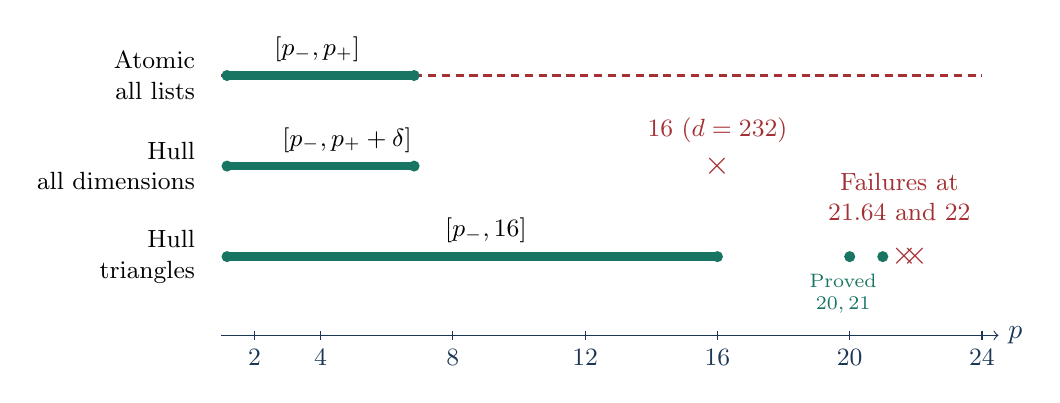
\begin{tikzpicture}[x=0.42cm,y=1cm]
 \draw[->,ink] (1,-3.3)--(24.5,-3.3) node[right]{$p$};
 \foreach \x in {2,4,8,12,16,20,24}
   \draw[ink] (\x,-3.24)--(\x,-3.36) node[below]{\small $\x$};
 \node[anchor=east,align=right,font=\small] at (0.5,0){Atomic\\all lists};
 \node[anchor=east,align=right,font=\small] at (0.5,-1.15){Hull\\all dimensions};
 \node[anchor=east,align=right,font=\small] at (0.5,-2.3){Hull\\triangles};
 \draw[proved,line width=3pt] (1.171573,0)--(6.828427,0);
 \draw[failure,densely dashed,thick] (1,0)--(1.171573,0);
 \draw[failure,densely dashed,thick] (6.828427,0)--(24,0);
 \draw[proved,line width=3pt] (1.171573,-1.15)--(6.828428,-1.15);
 \draw[proved,line width=3pt] (1.171573,-2.3)--(16,-2.3);
 \foreach \y in {0,-1.15,-2.3}
   \fill[proved] (1.171573,\y) circle (2pt);
 \fill[proved] (6.828427,0) circle (2pt);
 \fill[proved] (6.828428,-1.15) circle (2pt);
 \fill[proved] (16,-2.3) circle (2pt);
 \node[above,font=\small] at (3.9,0.05){$[\pn,\pp]$};
 \node[above,font=\small] at (4.8,-1.1){$[\pn,\pp+\delta]$};
 \node[above,font=\small] at (9,-2.25){$[\pn,16]$};
 \node[failure,font=\large] at (16,-1.15){$\times$};
 \node[above,font=\small,failure] at (16,-0.98){$16\ (d=232)$};
 \fill[proved] (20,-2.3) circle (2pt);
 \fill[proved] (21,-2.3) circle (2pt);
 \node[below,align=center,font=\scriptsize,proved] at (19.8,-2.4){Proved\\$20,21$};
 \node[failure,font=\large] at (21.64,-2.3){$\times$};
 \node[failure,font=\large] at (22,-2.3){$\times$};
 \node[above,align=center,font=\small,failure] at (21.5,-1.97){Failures at\\$21.64$ and $22$};
\end{tikzpicture}
\caption{Proved intervals (solid green), isolated proved endpoints
(green dots), and certified obstructions.
Atomic dashed portions are excluded by the exact classification. Hull
failure marks are individual exponents, not excluded half-lines. The tiny
common extension $\delta$ is not visually resolved at this scale. Blank
hull portions carry no positive or negative claim.}
\label{fig:ranges}
\end{figure}

\subsection{Minimal failure dimensions and upper failure powers}
\label{sec:dimensionprofile}
For proper simplices define
\[
 d_{\min}(p)=\min\{d\ge1:p\notin\mathcal A_d\},\qquad
 p_{\min}(d)=\inf\{p>4:p\notin\mathcal A_d\},
\]
with value $+\infty$ if the relevant set is empty. The second definition
concerns only the upper branch; it makes no connectedness assumption.
An explicit failure supplies an upper bound. A search that finds no
negative example supplies no global lower bound.

For each integer $p=7,8,9,10,11,12,13,14,15$, no failure witness was
found in the dimension investigation \cite{DimensionProfile}; no finite
upper bound on $d_{\min}(p)$ has been established. For $p=16$, the exact
result is \eqref{eq:232}. The triangle theorem gives $d_{\min}(p)\ge3$
when finite throughout these powers. In particular, $d_{\min}(7)$ is
unresolved: selected-family searches reaching dimension about one million
do not establish $d_{\min}(7)>10^6$ or $d_{\min}(7)=\infty$.

The main numerical construction groups $m=d-2$ copies of $A=(0,0,0)$,
one $B=(1,0,0)$, and two caps $(u,v,\pm c)$, $v,c>0$. Its projected law
is $\Dir(m,1,2)$. Every individual vertex type was tested, including
the mixed planar/transverse block of a cap response. A small regular
spread of the $A$ group in an orthogonal $(m-1)$-space gives a proper
$d$-simplex. At $p>4$, strict negative responses persist under sufficiently
small spreads by continuity. The numerical boundary uses the collapsed
limit to estimate onset; specified proper finite witnesses require the
additional error and spread control supplied by the exact certificates.

For noninteger powers the conditional cap integral is evaluated using
\[
 \E[(A+ZT^2)^q]=(A+Z)^q\,
 {}_2F_1\left(-q,1;\tfrac32;\frac Z{A+Z}\right),
 \qquad T\sim\operatorname{Unif}[-1,1].
\]
The second-$T$-moment replaces $3/2$ by $5/2$ and includes a factor $1/3$.
Positive Gaussian beta quadrature handles the remaining two integrals.
Orders $24$, $36$, and $52$ differed by less than $9.4\times10^{-10}$
in the scaled response minima at the reported failing powers. These are
numerical convergence checks, not interval enclosures.

\begin{table}[htbp]
\centering\small
\begin{tabular}{@{}rrr@{}}
\toprule
Intrinsic $d$ & Estimated onset & Numerically checked failing $p$\\
\midrule
$2$ & $21.6334$ & $21.7$\\
$3$ & $19.9547$ & $20.0$\\
$4$ & $19.5061$ & $19.6$\\
$5$ & $19.1657$ & $19.2$\\
$6$ & $18.8891$ & $18.9$\\
$8$ & $18.4589$ & $18.5$\\
$10$ & $18.1363$ & $18.2$\\
$12$ & $17.8844$ & $17.9$\\
$16$ & $17.5160$ & $17.6$\\
$20$ & $17.2597$ & $17.3$\\
$30$ & $16.8664$ & $16.9$\\
$50$ & $16.5007$ & $16.6$\\
$75$ & $16.2980$ & $16.3$\\
$100$ & $16.1911$ & $16.2$\\
$150$ & $16.0804$ & $16.1$\\
$200$ & $16.0236$ & $16.1$\\
$232$ & $15.9997$ & $16.0$\\
$250$ & $15.9890$ & $16.0$\\
$300$ & $15.9657$ & $16.0$\\
$500$ & $15.9187$ & $16.0$\\
$1{,}000$ & $15.8829$ & $15.9$\\
$10{,}000$ & $15.8504$ & $15.9$\\
$100{,}000$ & $15.8472$ & $15.9$\\
$1{,}000{,}000$ & $15.8469$ & $15.9$\\
\bottomrule
\end{tabular}
\caption{Numerical family onset and an actually checked negative power,
rounded upward to one decimal. These are not certified global values of
$p_{\min}(d)$. Exact results are identified in the text.}
\label{tab:dimensionprofile}
\end{table}
Dimension one has no failing power. Exact certificates already give
$p_{\min}(2)\le21.64$, $p_{\min}(3)\le20$, $p_{\min}(12)\le18$,
and $p_{\min}(232)\le16$. For example, $17.9$ at $d=12$ is a numerical
improvement on the exact witness at $18$; it is not presented as a new
exact certificate. Similarly, $16.5$ at $d=50$ would round \emph{below}
the estimated onset and is deliberately not listed as failing.

\begin{figure}[htbp]
\centering
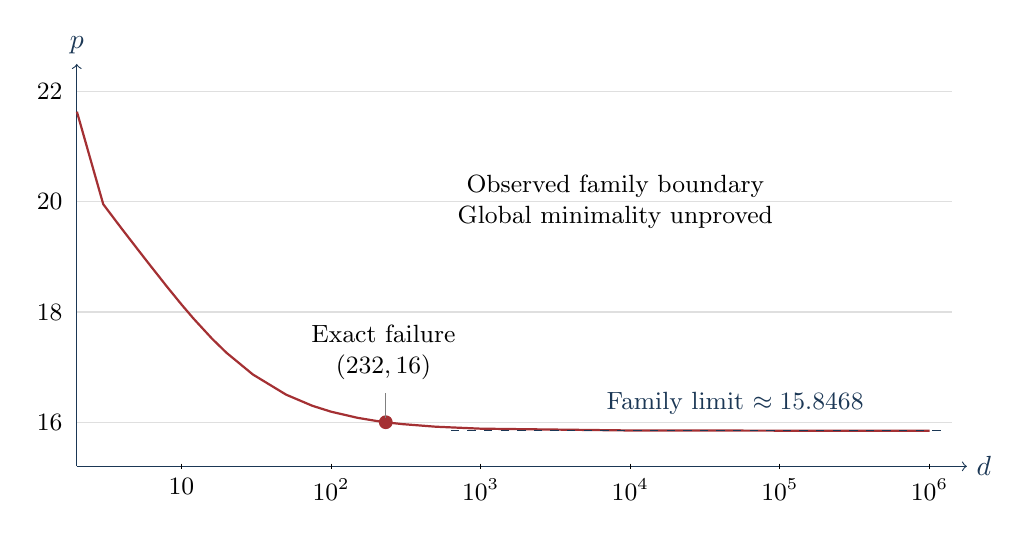
\begin{tikzpicture}[x=1.9cm,y=0.7cm]
 \foreach \p in {16,18,20,22} {
   \draw[gray!25] (0.3,\p)--(6.15,\p);
   \node[left,font=\small] at (0.27,\p){$\p$};
 }
 \draw[->,ink] (0.3,15.2)--(6.25,15.2) node[right]{$d$};
 \draw[->,ink] (0.3,15.2)--(0.3,22.5) node[above]{$p$};
 \foreach \x/\label in {1/10,2/10^2,3/10^3,4/10^4,5/10^5,6/10^6}
   \draw (\x,15.25)--(\x,15.15) node[below,font=\small]{$\label$};
 \draw[failure,thick] plot coordinates {
 (0.30103,21.6334) (0.477121,19.9547) (0.60206,19.5061)
 (0.69897,19.1657) (0.778151,18.8891) (0.90309,18.4589)
 (1,18.1363) (1.079181,17.8844) (1.20412,17.5160)
 (1.30103,17.2597) (1.477121,16.8664) (1.69897,16.5007)
 (1.875061,16.2980) (2,16.1911) (2.176091,16.0804)
 (2.30103,16.0236) (2.365488,15.9997) (2.39794,15.9890)
 (2.477121,15.9657) (2.69897,15.9187) (3,15.8829)
 (4,15.8504) (5,15.8472) (6,15.8469)};
 \draw[ink,dashed] (2.8,15.84681787)--(6.1,15.84681787);
 \node[ink,above,font=\small] at (4.7,15.97){Family limit $\approx15.8468$};
 \fill[failure] (2.365488,16) circle (2.5pt);
 \node[above,align=center,font=\small] at (2.35,16.6){Exact failure\\$(232,16)$};
 \draw[gray] (2.365488,16.08)--(2.365488,16.53);
 \node[align=center,font=\small] at (3.9,20){Observed family boundary\\Global minimality unproved};
\end{tikzpicture}
\caption{The numerical upper-failure family on a logarithmic dimension
axis. The connecting line guides the eye; it is not a global threshold
theorem. The dimension-$232$ mark has a separate exact finite certificate.}
\label{fig:dimensionprofile}
\end{figure}

Within this family the continuous multiplicity parameter crosses $p=16$
at dimension approximately $231.60314$: the optimized branch is positive
at $231$ and negative at $232$. Other families below $232$ are not excluded.
A separate exponential limiting-law calculation gives onset
$15.84681787$, consistent with the large finite-dimensional values.
There is no proof that this is $\lim_d p_{\min}(d)$, that this limit
exists, or that every dimension is attractive through $15$.

The compact follow-up searches comprised $50$ cluster-cap cases (all
integers $7$ through $16$ at $d=3,10,100,1000,10^6$), $96$ grouped
regular-fan cases, $18$ Gaussian/exponential limiting-law cases, and
$24$ asymmetric gamma/Gaussian cases, together with the boundary
continuations. Fan tests included the individual transverse cubic moments.
The general three-exponential search recovered the same limiting branch;
the other tested families did not lower it. Selected families and local
optimization cannot establish a global minimum or justify a
dimension-specific formula.

\section{Limiting centers, related mass models, and triangle Hearts}
As $p\downarrow1$, atomic power centers approach geometric medians when
the limiting median is unique; otherwise limiting minimizers lie in the
median set. On a triangle the Fermat construction is piecewise, depending
on its angles. The solid counterpart is a volume geometric median, a
different measure problem. No global hull-attractivity result is claimed
at $p=1$, outside the standing domain $p>1$.
At $p=\infty$ both supports lead to minimum-enclosing-ball centers, and
the acute circumcenter branch already has indefinite response. For
$C=(q,r)$ with $r>0$,
\[
 O(q,r)=\left(0,\frac{q^2+r^2-1}{2r}\right),\quad
 \det\Sym D_CO=-q^2/(4r^2)<0\quad(q\ne0).
\]
The exact finite large-power pair gives a separate quantitative realization.

Uniform boundary or skeletal mass is a further model. For the complete
$m$-skeleton of a proper $d$-simplex,
$C_{d,m}=\sum_F\Vol_m(F)c_F/\sum_F\Vol_m(F)$, where $c_F$ is a face
centroid. The extremes $m=0,d$ are the vertex centroid. Moving a vertex
changes both face locations and face masses, producing an extra
redistribution term in the derivative. For triangles the wire center is
$X(10)=((b+c)A+(c+a)B+(a+b)C)/(2(a+b+c))$, an attractive rule in the
prior theory. For the tetrahedron
$(0,0,0),(1,0,0),(0,1,0),(3,-2,1/2)$, both edge and face mass centers
have certified indefinite symmetric responses to movement of the second
vertex. They are not the uniform-solid hull-power model, even at quadratic
power, and cannot supply counterexamples to \eqref{eq:hull}.

The original finite triangle-center comparison also has a precise scope
\cite{PaperIII,Handoff}. Let $M_-=M_{\pn}$ and $M_+=M_{\pp}$.
The fixed $B46$ family retains these two maps and $44$ rational maps
($R44$). In the fixed $B76$ reference, neither endpoint is universally
contained in the convex hull of the other $75$ members. Certified support
separations occur at side triples $(4165,5213,1074)$ for $M_-$, with gap
$>26.18$, and $(268,499,321)$ for $M_+$, with gap $>4.99$.
The reported containment of all $1{,}142$ proved native ETC maps in
$\conv R44$ makes the same witnesses separate these endpoints from
that known native hull. Those are results for the specified finite
reference and its certificate archive, not exposedness on the unknown
maximal Heart, nor a proof that $B46$ is minimal or maximal.
The two endpoint values are also not proved to contain the whole curve
$p\mapsto M_p(P)$ in their convex hull.

The present hull-power maps on $[\pn,16]\cup\{20,21\}$ supply additional analytic,
similarity-equivariant attractive triangle maps. Fixed convex combinations
preserve these properties. Whether any of their values enlarge $B46$ or
are redundant has not been established. Also, convex combinations of
center maps do not equal intermediate members of a nonlinear power family;
they cannot replace the continuous exponent certificate.

\section{ETC neighbors and their independent attractivity}\label{sec:neighbors}
This section records a new comparison with the Encyclopedia of Triangle
Centers (ETC), using the numerical fingerprint method from the author's
\emph{Physically Inspired Triangle Centers} (PITC) project
\cite{PITC,Neighbors}. The ETC definitions retain the authorship of Clark
Kimberling and the Encyclopedia's contributors \cite{ETC}. All comparison
results, response investigations, and certificates in this section are
attributed to Ismail Hammoudeh, with extensive use of ChatGPT acknowledged.

\subsection{Comparison without a target barycentric formula}
For a target rule $Z$, solve its Cartesian position on each of $100$
training triangles $P_k$. Let $D_k$ be the longest side. The positional score
of an ETC rule $X_j$ is
\begin{equation}\label{eq:etc-rms}
 E_{\rm train}(Z,X_j)=\left(\frac1{100}\sum_{k=1}^{100}
 \frac{\|Z(P_k)-X_j(P_k)\|^2}{D_k^2}\right)^{1/2}.
\end{equation}
The triangles are PITC's fixed equal-area grid in triangle-angle shape
space. A separate $40$-triangle holdout supplies validation RMS and maximum
errors; it is not used to rerank candidates. Thus no symbolic barycentric
function for $M_p$ or $U_p$ is needed. ``Nearest'' means nearest under this
specified finite fingerprint, not nearest for every individual triangle.

The supplied snapshot has $72{,}807$ records. All were visited, but only
$70{,}853$ have complete finite evaluable fingerprints on the training
grid. The other $1{,}954$ are excluded for unsupported symbols or
nonfinite values. Unused zero-filled cache rows are not candidates.
The result is therefore a ranking within this evaluable snapshot, not a
claim about every ETC entry currently available online. Its database
SHA256 is
\begin{quote}\footnotesize
\pathcode{ace501d40dd83785f89b4de8e4ddcc0c5081d82de82e1baf37816d10e547cbfa}.
\end{quote}

We compare $33$ selected powers in $1<p<25$, including $65/64$, $\pn$,
$21.63$, and $24.99$. On the $140$ training and validation shapes, all
$4{,}620$ pairs of power-center solves resolve. Hull quadrature orders $40$
and $64$ differ by at most $3.80\times10^{-12}$ times the triangle diameter
on this data set. This is a floating-point consistency check, not a
rigorous integration error certificate. For obtuse triangles near $p=1$,
atomic solves use a generalized Weiszfeld majorization before Newton
iteration to handle centers very close to a vertex.

At $p=2$, both target rules are exactly $X(2)$, the centroid. At $p=4$,
the leading atomic match is $X(15810)$, with training and validation RMS
errors $0.1257\%$ and $0.1322\%$ of diameter; the leading hull match is
$X(52788)$, with errors $0.2038\%$ and $0.2080\%$. Proximity at the other
powers establishes neither an identity nor a barycentric formula for
the target. The full scores and maximum errors are distributed with
\pathcode{explorer/data/etc-matches.csv}.

\subsection{A separate attractivity investigation}
An ETC rule has no power parameter here. Its response status belongs to
the rule and does not change when it is shortlisted at a different $p$.
For every selected formula, forward automatic differentiation computes
the three $2\times2$ vertex Jacobians. We screen their symmetric parts on
$983$ proper triangles: the $140$ fingerprint triangles, $700$ seeded
random shapes with apex coordinates in $[-0.8,1.8]$ and logarithmically
distributed heights in $[0.002,3]$, and $143$ thin, obtuse, right, and
isosceles family members. All $85$ included formulas, including three
additional baseline rules, are finite on all these shapes.

Negative differential responses are converted into finite motions.
Rational interval arithmetic then verifies proper before/after triangles,
nonzero homogeneous weight sums, and a strictly negative upper endpoint
for $h\cdot(X(P_{i,h})-X(P))$. Square roots are enclosed using integer square
root on a rational grid with $45$ decimal places; subsequent arithmetic
uses exact fractions. There are $34$ certified failures in the full
formula set, of which $33$ are actual shortlisted neighbors; the extra
failure is baseline $X(6)$.

Among the $82$ distinct shortlisted neighbors, $33$ are therefore proved
nonattractive, $3$ are proved attractive by the arguments below, and $46$
have no sampled failure but no all-shape proof in this investigation.
Small nonnegative sampled eigenvalues do not certify a positive lower
bound over all shapes. The response CSV and exact interval records are
\pathcode{explorer/data/etc-attractivity.csv} and
\pathcode{explorer/data/etc-attractivity-certificates.json}.

\subsection{An algebraic counterexample for a hull neighbor}
\begin{proposition}\label{prop:neighbor-negative}
The ETC rule $X(7934)$ is not vertex-attractive, although it is the leading
fingerprint match for the universally attractive triangle hull-power
center $U_{12}$.
\end{proposition}
\begin{proof}
The ETC barycentrics of $X(7934)$ are the cyclic values of
\[
 f(a,b,c)=2b^4-b^2c^2+2c^4.
\]
Let $A=(0,0)$, $B=(1,0)$, $C=(1/2,t)$ and put $q=1/4+t^2$.
The weights at $A,B,C$ are respectively
$2q^2-q+2$, $2q^2-q+2$, and $3q^2$. Differentiate after moving $C$
horizontally. The total weight has derivative zero at this symmetric
shape, and the horizontal response is
\begin{equation}\label{eq:7934-negative}
 \frac{\partial X_x(7934)}{\partial C_x}
 =\frac{3q^2-4q+1}{7q^2-2q+4}
 =\frac{(3q-1)(q-1)}{7q^2-2q+4}.
\end{equation}
It is negative whenever $1/3<q<1$, equivalently
$1/12<t^2<3/4$. At $t=5/8$, $q=41/64$ and the derivative is
$-1357/22903$. There is also an exact finite witness: with
$h=(1/1000,0)$ applied to $C$, direct rational evaluation of the squared
side lengths gives
\[
 h\cdot\bigl(X(7934;A,B,C+h)-X(7934;A,B,C)\bigr)
 =-\frac{82823496093}{1397892175783000000}<0.
\]
Both endpoint triangles are proper. The fingerprint match at $p=12$
has training RMS $1.2287\%$ and holdout RMS $1.1196\%$ of diameter.
The independent all-shape proof for $U_{12}$ remains valid.
\end{proof}

At $p=14$ the three hull neighbors $X(7934),X(7911),X(32578)$ all have
certified failures. At $p=16$ the three are
$X(7911),X(25682),X(7934)$, again all failing. At $p=20$, $21$, and
$21.63$, the three are $X(25682),X(7911),X(7910)$, all failing.
In particular, the proved hull endpoints $16$, $20$, and $21$ cannot
transfer attractivity to their positional neighbors. The branch estimate
$21.63336$ supplies no such implication either.

\subsection{Positive algebraic certificates for two neighbors}
\begin{proposition}\label{prop:neighbor-positive}
The ETC rules $X(18236)$ and $X(56203)$ satisfy finite vertex attractivity
for every motion with proper triangle endpoints. In particular,
$X(18236)$ is an attractive leading neighbor of $M_7$, even though
$7>4+2\sqrt2$ and $M_7$ is not universally attractive.
\end{proposition}
\begin{proof}
Their first homogeneous barycentric polynomials are
\begin{align*}
 f_{18236}(a,b,c)&=a(a-b-c)\,g(a,b,c),\\
 g(a,b,c)&=a^3b-a^2b^2-ab^3+b^4+a^3c-2a^2bc+3ab^2c+2b^3c\\
 &\quad-a^2c^2+3abc^2-6b^2c^2-ac^3+2bc^3+c^4,\\
 f_{56203}(a,b,c)&=a(a-b-c)(2a+2b+c)(2a+b+2c).
\end{align*}
Here $a=|B-C|$, $b=|C-A|$, $c=|A-B|$. The following reduction
and its exact coefficient lists provide a finite sufficient certificate.
For either $f$, write
\[
 W_A=f(a,b,c),\quad W_B=f(b,c,a),\quad W_C=f(c,a,b),\quad
 T=W_A+W_B+W_C.
\]
Place $A=(0,0)$, $B=(c,0)$, $C=(x,y)$, so that
$x=(b^2+c^2-a^2)/(2c)$ and $y^2=b^2-x^2$. Define polynomials
\[
 U_k=c\bigl((\partial_kW_B)T-W_B\partial_kT\bigr),\quad
 L_k=(\partial_kW_C)T-W_C\partial_kT,\qquad k=a,b.
\]
Set $z=b^2+c^2-a^2$, $\tau=b^2-c^2-a^2$,
$Y=4b^2c^2-z^2$, and
\begin{align*}
 N_x&=4abc^2TW_C+2bcU_a\tau+2acU_bz+ bzL_a\tau+az^2L_b,\\
 N_y&=4abc^2TW_C+Y(bL_a+aL_b),\\
 N_o&=2bc^2U_a+2ac^2U_b+bc(z+\tau)L_a+2aczL_b.
\end{align*}
Direct differentiation of
$X_x=(cW_B+xW_C)/T$, $X_y=yW_C/T$ gives, for
$K=\Sym D_CX$ and $F=4abc^2T^2$,
\[
 K_{xx}=N_x/F,\qquad K_{yy}=N_y/F,\qquad K_{xy}=yN_o/F,
 \qquad \det K=\frac{4c^2N_xN_y-YN_o^2}{4c^2F^2}.
\]
Substitute $a=v+w$, $b=w+u$, $c=u+v$. Every proper triangle
corresponds to $u,v,w>0$. Exact polynomial expansion gives strictly
positive coefficients for every nonzero term of $N_y$, of
$4c^2N_xN_y-YN_o^2$, and of $T^2$. The respective numbers of terms
are
\begin{center}
\begin{tabular}{lrrr}
\toprule Rule & $N_y$ & determinant numerator & $T^2$\\\midrule
$X(18236)$ & 95 & 363 & 61\\
$X(56203)$ & 60 & 266 & 36\\\bottomrule
\end{tabular}
\end{center}
Consequently $T\ne0$, $K_{yy}>0$, and $\det K>0$ on proper
triangles. One positive diagonal and a positive determinant imply
$K\succ0$; no separate positive-coefficient expansion of $N_x$ is
needed. Cyclic relabeling proves the same property for each moved vertex.
The exact expansions are distributed in
\pathcode{explorer/data/etc-positive-certificates.json} and regenerated
by \pathcode{research/etc_matching/prove_positive.py}, which uses only
integer and rational sparse polynomial arithmetic.

The $T^2$ expansions also contain a positive term on each open boundary
face $u=0$, $v=0$, or $w=0$. Thus the formulas remain defined and
continuous at every distinct collinear triangle, and their response
matrices there are positive semidefinite by continuity. Integrating the
local response along a single-vertex segment which avoids coincidences
gives the finite inequality. A segment through a coincidence can be
approximated by segments avoiding it, keeping its two proper endpoints
arbitrarily close to the original endpoints. Continuity at those
endpoints then gives the finite inequality in the limit. No prescribed
value at an exactly coincident input is asserted for these two ETC
formulas.
\end{proof}

The leading $p=7$ atomic shortlist is
$X(18236),X(30624),X(46844)$. The first rule has the positive proof just
given, while the latter two have exact finite failures. The leading
match has holdout RMS $1.1433\%$ of diameter. Thus failure of $M_p$
above its universal interval does not force failure of its neighboring
ETC rules. X(56203), for example a hull neighbor at $p=8$, supplies a
second positive all-shape certificate. Together with the centroid's
exact response $D_{v_i}X(2)=I/3$, these are the three accepted positive
neighbor results. The remaining numerical passes stay unproved.

\subsection{All selected powers and the explorer}
In the following table the three ETC numbers are ordered by training
RMS. Superscript $A$ means proved attractive (the proper-endpoint scope
above applies to $18236$ and $56203$); $F$ means certified finite failure;
$?$ means no sampled failure and no all-shape proof. These are statuses
of ETC rules, not new statements about the corresponding target powers.
\begin{table}[p]
\centering\small
\caption{ETC fingerprint neighbors and independent response status.}\label{tab:etc-neighbors}
\begin{tabular}{@{}r|rrr|rrr@{}}
\toprule $p$ & \multicolumn{3}{c|}{Atomic neighbors} & \multicolumn{3}{c}{Hull neighbors}\\\midrule
$1.01$ & $54788^{F}$ & $11544^{F}$ & $1996^{F}$ & $55759^{?}$ & $63120^{?}$ & $31312^{?}$\\
$65/64$ & $60083^{F}$ & $11544^{F}$ & $1996^{F}$ & $55759^{?}$ & $55758^{?}$ & $63120^{?}$\\
$1.05$ & $7272^{F}$ & $60258^{F}$ & $60617^{F}$ & $55758^{?}$ & $4798^{?}$ & $51126^{?}$\\
$1.1$ & $42321^{F}$ & $56929^{F}$ & $4059^{F}$ & $4798^{?}$ & $51126^{?}$ & $55757^{?}$\\
$\pn$ & $61013^{F}$ & $61027^{F}$ & $62919^{F}$ & $60644^{?}$ & $55756^{?}$ & $55755^{?}$\\
$1.25$ & $62921^{F}$ & $30380^{F}$ & $57722^{F}$ & $55754^{?}$ & $6707^{?}$ & $55755^{?}$\\
$1.5$ & $60096^{?}$ & $60204^{?}$ & $36511^{?}$ & $55750^{?}$ & $55751^{?}$ & $62940^{?}$\\
$2$ & $2^{A}$ & $51553^{?}$ & $53004^{?}$ & $2^{A}$ & $51553^{?}$ & $53004^{?}$\\
$2.5$ & $7944^{?}$ & $5599^{?}$ & $17250^{?}$ & $61001^{?}$ & $19872^{?}$ & $31253^{?}$\\
$3$ & $69642^{?}$ & $3305^{?}$ & $54357^{?}$ & $31268^{?}$ & $15894^{F}$ & $52706^{?}$\\
$4$ & $15810^{?}$ & $56508^{?}$ & $29492^{?}$ & $52788^{?}$ & $46225^{?}$ & $7914^{?}$\\
$5$ & $7928^{F}$ & $15810^{?}$ & $32578^{F}$ & $7937^{?}$ & $5506^{?}$ & $5316^{?}$\\
$6$ & $46844^{F}$ & $18236^{A}$ & $50219^{F}$ & $7853^{?}$ & $31246^{?}$ & $24954^{?}$\\
$7$ & $18236^{A}$ & $30624^{F}$ & $46844^{F}$ & $7853^{?}$ & $7935^{?}$ & $24707^{?}$\\
$8$ & $30624^{F}$ & $18236^{A}$ & $40175^{F}$ & $24707^{?}$ & $7935^{?}$ & $56203^{A}$\\
$9$ & $40175^{F}$ & $30624^{F}$ & $15855^{F}$ & $7831^{?}$ & $24707^{?}$ & $56203^{A}$\\
$10$ & $40175^{F}$ & $15855^{F}$ & $59646^{F}$ & $7831^{?}$ & $29492^{?}$ & $56508^{?}$\\
$11$ & $40175^{F}$ & $15855^{F}$ & $59646^{F}$ & $7831^{?}$ & $29492^{?}$ & $56508^{?}$\\
$12$ & $40175^{F}$ & $15855^{F}$ & $31594^{F}$ & $7934^{F}$ & $15810^{?}$ & $56508^{?}$\\
$13$ & $40175^{F}$ & $15855^{F}$ & $31594^{F}$ & $7934^{F}$ & $7911^{F}$ & $15810^{?}$\\
$14$ & $40175^{F}$ & $15855^{F}$ & $6554^{F}$ & $7934^{F}$ & $7911^{F}$ & $32578^{F}$\\
$15$ & $40175^{F}$ & $15855^{F}$ & $6554^{F}$ & $7911^{F}$ & $7934^{F}$ & $25682^{F}$\\
$16$ & $40175^{F}$ & $6554^{F}$ & $15855^{F}$ & $7911^{F}$ & $25682^{F}$ & $7934^{F}$\\
$17$ & $40175^{F}$ & $6554^{F}$ & $15855^{F}$ & $25682^{F}$ & $7911^{F}$ & $7934^{F}$\\
$18$ & $40175^{F}$ & $6554^{F}$ & $15855^{F}$ & $25682^{F}$ & $7911^{F}$ & $7910^{F}$\\
$19$ & $6554^{F}$ & $40175^{F}$ & $15855^{F}$ & $25682^{F}$ & $7911^{F}$ & $7910^{F}$\\
$20$ & $6554^{F}$ & $40175^{F}$ & $15855^{F}$ & $25682^{F}$ & $7911^{F}$ & $7910^{F}$\\
$21$ & $6554^{F}$ & $40175^{F}$ & $5574^{F}$ & $25682^{F}$ & $7911^{F}$ & $7910^{F}$\\
$21.63$ & $6554^{F}$ & $40175^{F}$ & $5574^{F}$ & $25682^{F}$ & $7911^{F}$ & $7910^{F}$\\
$22$ & $6554^{F}$ & $40175^{F}$ & $5574^{F}$ & $25682^{F}$ & $7911^{F}$ & $7910^{F}$\\
$23$ & $6554^{F}$ & $5574^{F}$ & $40175^{F}$ & $25682^{F}$ & $7911^{F}$ & $7910^{F}$\\
$24$ & $5574^{F}$ & $6554^{F}$ & $9713^{F}$ & $25682^{F}$ & $7911^{F}$ & $7910^{F}$\\
$24.99$ & $5574^{F}$ & $6554^{F}$ & $9713^{F}$ & $25682^{F}$ & $40175^{F}$ & $7911^{F}$\\
\bottomrule
\end{tabular}
\end{table}

The free browser explorer at
\href{https://ismaa3iil.fyi/power-centers-explorer/}{ismaa3iil.fyi/power-centers-explorer/}
now offers all $33$ comparisons, overlays of either or both shortlists,
training, validation, and current-triangle distances, and separate
response-status labels. ``Show failure'' loads a certified triangle;
the stored motion can be applied and reset. Displayed positions and
local response values remain floating-point diagnostics; the downloadable
exact records support the proof labels. Arbitrary powers between the
sampled values do not receive interpolated rankings. The triangle range
is $[1.01,24.99]$ and the tetrahedron range remains $[\pn,19.95]$.
ETC comparisons concern triangles only. The explorer uses free local
JavaScript tools and includes only selected formulas, not the full
database. Proximity never changes the attractivity claims proved in
earlier sections, nor certifies all $p<21.63$ for $U_p$.


\section{Reproducibility and the status of the proofs}
The analytic arguments and the finite certificate data have different
roles. The common dimension-independent extension is proved by the
exponential-moment and matrix estimates; its small constant checker verifies
the displayed rational margins. The triangle theorem additionally depends
on complete finite covers and exact arithmetic replay. Floating calculations
propose boxes, center guesses, and preconditioners. They make no acceptance
decision in the final proof. Exact finite counterexamples include both
integration error and residual-to-center error. Numerical searches guide
the investigation and carry no all-shape positivity conclusion.

All exact replay programs use ordinary Python 3 with its standard library.
They must run without \texttt{-O}, because assertions are part of the
verification. The \texttt{-S} option demonstrates independence from installed
packages. Construction and exploratory numerical searches require NumPy.
Useful commands from the workspace root are:
\begin{quote}\footnotesize\ttfamily
python -S research/verify\_positive\_bound.py\\
python -S research/triangle8\_interval.py --replay\\
python -S research/triangle10\_interval.py --replay\\
python -S research/triangle12\_interval.py --replay\\
python -S research/triangle\_extended\_integer.py --power 16 --workers 4\\
python -S research/triangle\_extended\_integer.py --power 20 --workers 4\\
python -S research/triangle\_extended\_integer.py --power 21 --workers 4\\
python -S research/triangle\_power\_integer\_replay.py --workers 4\\
python -S research/triangle\_extended\_integer.py --power 16 --continuous --workers 4\\
python -S research/verify\_dimension232.py\\
python -S research/downward\_closure\_countercheck.py
\end{quote}
The $p=16$ endpoint replay checks $74{,}996$ leaves, depth $20$.
The continuous $[10,16]$ replay checks $3{,}042{,}242$ leaves, depth $28$;
its completed eight-worker run took approximately $7{,}939$ seconds on the
investigation machine. Worker counts affect runtime, not the mathematical
tests. Streaming workers retain at most $128$ proposals at a time, while
the parent audits the full cover and verifies each worker input hash and
record count. Independent moment and interval-primitive cross-checks
support the implementation; none substitutes for the complete replay.

Four principal certificate SHA256 values are
\begin{quote}\footnotesize
Endpoint $p=16$:\\*
\pathcode{52ee00ac65cb6601a88e5c144cd2fb8e238b3f624a7da87d434ee4c87ec98c6e}\\[3pt]
Continuous $[10,16]$:\\*
\pathcode{59046abff6f15c663f2c8a5b287f33565f9187915458f714c35b1cbe977fb0d6}\\[3pt]
Endpoint $p=20$:\\*
\pathcode{d18f39bf441fb16b9b7465f4264eceb60281a9cf7ad1ccb3245f764aec660fab}\\[3pt]
Endpoint $p=21$:\\*
\pathcode{20b338bf9d4fbc4027e970297c2acd85e8a75bf374844eb44eebd609f2499dbc}
\end{quote}
The focused distribution is
\pathcode{Triangle16_ContinuousInterval_Certificates_2026-10-03.zip}.
It passed archive integrity and file-hash checks and independent validators
run from an extracted copy. Its SHA256 is
\begin{quote}\footnotesize
\pathcode{bb545adce451cee7f76932b350c9a292997359902ac6d8a78272641ef9e8e4a1}.
\end{quote}
The full investigation distribution is
\pathcode{Hull_Power_Investigation_Triangle16_Interval_2026-10-03.zip};
its verified SHA256 is
\begin{quote}\footnotesize
\pathcode{152a6816eaac408c3ed20ac5d72f815fad01dc8ec5ae7e47633f1ef4354084eb}.
\end{quote}
The later focused distributions are
\pathcode{Triangle20_LowPower_Certificates_2026-10-03.zip} and
\pathcode{Triangle21_Endpoint_Certificates_2026-10-03.zip}.
The final-statement records pin endpoint source and replay hashes.
The dimension-$232$ certificate separately pins its exact-moment dependencies.
No completed complete-cover replay for $[16,21]$ is included among the
accepted records as of this revision. Partial continuation work is not
counted as an interval theorem.

For this rewritten article, an editorial audit compares table entries,
rational margins, and cited paths against the accepted records. It does
not rerun the multi-million-box proofs. Analytic structural results have
their proofs above and in the cited notes; the associated floating-point
diagnostics are labeled separately. Existing certificate archives are
preserved. This article supplies neither a sharp cutoff nor a global
dimension formula.

\section{Remaining mathematical questions}
The central triangle problem is to connect the continuous interval through
$16$ with the separately certified endpoints $20$ and $21$. A complete
shape/exponent certificate over $[16,21]$ or a proof of all-shape downward
closure would do so. The exact crossing identity \eqref{eq:crossing}
isolates a sufficient sign inequality; its universal sign remains open.
Fixed-triangle and fixed-motion no-re-entry are false and cannot supply
that proof. Existence, uniqueness, and eventual failure of the projective
families do not establish persistence from the first failure.

The observed triangle branch near $21.63336$ needs a global exclusion of
other shapes and branches before it can be called sharp. The lower
hull-power interval $(1,\pn)$ also remains unclassified. In particular,
the local certificates and positive search evidence at $65/64$ do not
settle its all-shape question; atomic necessity does not transfer.

For tetrahedra, all-shape certificates at $16$ or $18$ would convert strong
search evidence into theorems. Further proper higher-dimensional families,
all-vertex response tests, and sharper analytic common bounds are needed
to identify dimension dependence globally. The dimension-$232$ witness
improves the upper bound for $d_{\min}(16)$, but a smaller failure dimension
is not excluded. For each integer $7$ through $15$, no finite failure
dimension is established. The observed limit $15.8468$ belongs to the
examined family and is not a dimension-independent sharp endpoint.

Connectedness of the \emph{all-shape} attractive sets, upward persistence
of the existence of some bad simplex, and nesting across intrinsic
dimensions all remain open. These are distinct from the disproved
fixed-shape no-re-entry assertion.
The small common extension $\delta$ reflects conservative estimates rather
than a proved near-band obstruction. Finally, a certified support comparison
of hull-power triangle maps with $B46$ is separate from the attractivity
problem and remains to be carried out.

\appendix
\section{Source and certificate inventory}
All paths below are relative to the workspace root; the standalone article
has no compilation dependency on them.\par\medskip
\begingroup\small\raggedright
\noindent\textbf{Atomic classification, radial theory, continuum consistency}\par\nopagebreak[4]
\pathcode{bundle/simplex_integral_power_centers_handoff_2026-10-01/paper/Attractive_Centers_III_v2.tex}\par\medskip
\noindent\textbf{Transfer, proper analyticity, quartic moments, large-power pair}\par\nopagebreak[4]
\pathcode{bundle/simplex_integral_power_centers_handoff_2026-10-01/POWER_CENTERS_AND_UNIFORM_SIMPLEX_HANDOFF.md}\par\medskip
\noindent\textbf{Concrete atomic and skeletal witnesses}\par\nopagebreak[4]
\pathcode{bundle/simplex_integral_power_centers_handoff_2026-10-01/existing_certificates/verify_interval_certificates.py}\par\medskip
\noindent\textbf{Every-dimensional positive extension}\par\nopagebreak[4]
\pathcode{research/ALL_SHAPE_AND_DIMENSION.md}\par
\pathcode{research/verify_positive_bound.py}\par\medskip
\noindent\textbf{Triangle $8,10,12,16$ endpoints}\par\nopagebreak[4]
\pathcode{research/triangle8_interval.py}\par
\pathcode{research/triangle10_interval.py}\par
\pathcode{research/triangle12_interval.py}\par
\pathcode{research/triangle_extended_integer.py}\par\medskip
\noindent\textbf{Continuous triangle intervals}\par\nopagebreak[4]
\pathcode{research/triangle_power_integer_replay.py}\par
\pathcode{research/triangle_extended_integer.py}\par
\pathcode{research/triangle_commutator_response.py}\par\medskip
\noindent\textbf{Triangle $20,21$ endpoints and low power}\par\nopagebreak[4]
\pathcode{research/TRIANGLE20_AND_LOW_POWER.md}\par
\pathcode{research/TRIANGLE21_ENDPOINT.md}\par
\pathcode{research/certify_triangle65_64.py}\par
\pathcode{research/verify_atomic65_64.py}\par\medskip
\noindent\textbf{Endpoint replay records}\par\nopagebreak[4]
\pathcode{research/triangle20_endpoint_integer_replay.json}\par
\pathcode{research/triangle21_endpoint_integer_replay.json}\par\medskip
\noindent\textbf{Triangle finite failures}\par\nopagebreak[4]
\pathcode{research/verify_rational_power.py}\par
\pathcode{research/verify_p22_finite.py}\par\medskip
\noindent\textbf{Tetrahedron and proper dimensions $5,31$}\par\nopagebreak[4]
\pathcode{research/verify_tetra20.py}\par
\pathcode{research/verify_dimension5_p20.py}\par
\pathcode{research/verify_dimension31.py}\par\medskip
\noindent\textbf{Proper dimensions $12,302$}\par\nopagebreak[4]
\pathcode{research/verify_cluster_caps_finite.py}\par
\pathcode{research/cluster_caps_finite_certificates.json}\par\medskip
\noindent\textbf{Proper dimension $232$}\par\nopagebreak[4]
\pathcode{research/verify_dimension232.py}\par
\pathcode{research/dimension232_certificate.json}\par\medskip
\noindent\textbf{Fixed-triangle and fixed-motion re-entry}\par\nopagebreak[4]
\pathcode{research/DOWNWARD_CLOSURE_COUNTERCHECK.md}\par
\pathcode{research/downward_closure_countercheck.py}\par\medskip
\noindent\textbf{Downward closure, disk test, projective families}\par\nopagebreak[4]
\pathcode{research/EXPONENT_DOWNWARD_CLOSURE.md}\par
\pathcode{research/DOWNWARD_CLOSURE_PROJECTIVE_REDUCTION.md}\par\medskip
\noindent\textbf{Crossing diagnostics}\par\nopagebreak[4]
\pathcode{research/validate_downward_projective_reduction.py}\par
\pathcode{research/downward_crossing_probe_roots.json}\par\medskip
\noindent\textbf{Dimension/power profile}\par\nopagebreak[4]
\pathcode{research/DIMENSION_FAILURE_PROFILE.md}\par
\pathcode{research/dimension_failure_profile.json}\par
\pathcode{research/dimension16_improvement.json}\par\medskip
\noindent\textbf{Triangle, tetrahedron, higher-dimensional searches}\par\nopagebreak[4]
\pathcode{research/global_triangle_search.py}\par
\pathcode{research/tetra_global_search.py}\par
\pathcode{research/higher_proper_search.py}\par
\pathcode{research/cluster_caps_search.py}\par\medskip
\noindent\textbf{ETC fingerprint comparisons and neighbor proofs}\par\nopagebreak[4]
\pathcode{research/etc_matching/build_inputs.py}\par
\pathcode{research/etc_matching/compute_centers.mjs}\par
\pathcode{research/etc_matching/rank.py}\par
\pathcode{research/etc_matching/screen_attractivity.mjs}\par
\pathcode{research/etc_matching/certify_neighbors.py}\par
\pathcode{research/etc_matching/prove_positive.py}\par\medskip
\endgroup

\begin{thebibliography}{99}
\bibitem{PaperIII}
Ismail Hammoudeh, \emph{Attractive Centers III: Radial Location Functionals,
Mechanical Response, and an Exact Elasticity Classification}, Version 2,
1 October 2026. Supplied manuscript and certificate records.
\bibitem{Handoff}
Ismail Hammoudeh, \emph{Power Centers and the Uniform-Simplex Modification}, research handoff,
1 October 2026. Local source identified in the appendix.
\bibitem{FirstInvestigation}
Ismail Hammoudeh, \emph{Hull-Power-Centers: First Attractivity Investigation},
1 October 2026, \pathcode{research/INVESTIGATION.md}.
\bibitem{DimensionReport}
Ismail Hammoudeh, \emph{All-Shape Positivity and Dimension Dependence of Hull-Power-Centers},
1 October 2026, with continuation notices through 3 October,
\pathcode{research/ALL_SHAPE_AND_DIMENSION.md}.
\bibitem{Triangle8}
Ismail Hammoudeh, \emph{Triangle $p=8$ Certificate and Proper Higher-Dimensional Failures},
2 October 2026, \pathcode{research/TRIANGLE8_AND_GLOBAL_SEARCH.md}.
\bibitem{Triangle10}
Ismail Hammoudeh, \emph{All-Shape Triangle Attractivity at $p=10$}, 2 October 2026,
\pathcode{research/TRIANGLE10_ALL_SHAPE.md}.
\bibitem{Triangle12}
Ismail Hammoudeh, \emph{Triangle Hull-Power Centers: $p=12$ and a Continuous Exponent Interval},
2 October 2026, with a later-result notice on 3 October,
\pathcode{research/TRIANGLE12_AND_CONTINUOUS_INTERVAL.md}.
\bibitem{Triangle16}
Ismail Hammoudeh, \emph{Triangle Hull-Power Centers at $p=16$ and over a Continuous Interval},
3 October 2026, \pathcode{research/TRIANGLE16_AND_CONTINUOUS_INTERVAL.md},
and the completed endpoint and continuation integer replay records.
\bibitem{Triangle20}
Ismail Hammoudeh, \emph{Triangle Hull-Power Centers at $p=20$ and $p=65/64$},
3 October 2026, \pathcode{research/TRIANGLE20_AND_LOW_POWER.md},
with exact endpoint, local low-power, and atomic certificate records.
\bibitem{Triangle21}
Ismail Hammoudeh, \emph{All-Shape Triangle Hull-Power Attractivity at $p=21$},
3 October 2026, \pathcode{research/TRIANGLE21_ENDPOINT.md},
with the completed independent integer replay.
\bibitem{Downward}
Ismail Hammoudeh, \emph{Does an Attractive Upper Exponent Force Every Lower
Exponent above Four?}, revised 5 October 2026,
\pathcode{research/EXPONENT_DOWNWARD_CLOSURE.md}.
\bibitem{Countercheck}
Ismail Hammoudeh, \emph{Fixed-Triangle No-Re-Entry Is False},
4--5 October 2026, \pathcode{research/DOWNWARD_CLOSURE_COUNTERCHECK.md},
with its exact polynomial certificate and asymptotic proof.
\bibitem{Projective}
Ismail Hammoudeh, \emph{Downward Closure: A Projective Comparison and a Disk
Criterion}, revised 5 October 2026,
\pathcode{research/DOWNWARD_CLOSURE_PROJECTIVE_REDUCTION.md}.
\bibitem{DimensionProfile}
Ismail Hammoudeh, \emph{Numerical Failure Dimensions and Powers for
Hull-Power Centers}, 5 October 2026,
\pathcode{research/DIMENSION_FAILURE_PROFILE.md}, with the exact
dimension-$232$ certificate and numerical search records.
\bibitem{Neighbors}
Ismail Hammoudeh, \emph{ETC Neighbors of Power Centers and Hull-Power Centers:
Fingerprint Rankings and Independent Attractivity Certificates},
6 October 2026, \pathcode{research/ETC_NEIGHBORS.md}, with the numerical
rankings, exact finite failures, and positive polynomial coefficient records.
\bibitem{PITC}
Ismail Hammoudeh, \emph{Triangle Centers Inspired by Physics}, PITC project,
3 October 2026; numerical ETC comparison protocol and supplied database snapshot.
\href{https://ismaa3iil.fyi/}{Author's research website}.
\bibitem{ETC}
Clark Kimberling and contributors, \emph{Encyclopedia of Triangle Centers}.
\href{https://faculty.evansville.edu/ck6/encyclopedia/etc.html}{Official online encyclopedia},
including the entries X(7934), X(18236), and X(56203); accessed 6 October 2026.
\bibitem{AGN}
Ben Andrews, Pengfei Guan, and Lei Ni,
\emph{Flow by Powers of the Gauss Curvature},
Advances in Mathematics \textbf{299} (2016), 174--201.
\href{https://doi.org/10.1016/j.aim.2016.05.008}{doi:10.1016/j.aim.2016.05.008}.
\end{thebibliography}
\end{document}
